% ---------------------------------------------------------
% Semester Project Report (Final Polished Version - Updated)
% Author: Ayush Raj, Roll No: 20221068
% Supervisor: Dr. Bedartha Goswami
% Department of Data Science, IISER Pune
% Date: November 20, 2025
% ---------------------------------------------------------

\documentclass[12pt]{report}
\usepackage[utf8]{inputenc}
\usepackage[T1]{fontenc}
\usepackage{graphicx,caption,subcaption,float}
\usepackage{amsmath,amssymb,amsfonts}
\usepackage{geometry}
\usepackage{setspace}
\usepackage{microtype}
\usepackage{parskip}
\usepackage{hyperref}
\usepackage{cite}
\usepackage{placeins}
\usepackage{adjustbox}
\usepackage{verbatim} % for verbatim blocks

\geometry{margin=1in}
\setstretch{1.15}

\captionsetup{font=small,labelfont=bf,skip=6pt}
\captionsetup[sub]{font=footnotesize,labelfont=bf,skip=4pt}

% Reduce float spacing
\setlength{\textfloatsep}{10pt}
\setlength{\floatsep}{8pt}
\setlength{\intextsep}{8pt}

\begin{document}

% ---------------------------------------------------------
% Title Page (Improved, tighter, same structure)
% ---------------------------------------------------------
\begin{titlepage}
\centering

\vspace*{0.4cm}
\includegraphics[width=0.27\textwidth]{logo.png}\\[1cm]

{\Large Indian Institute of Science Education and Research (IISER) Pune}\\[4pt]
{\large Department of Data Science}\\[1.2cm]

{\Huge\bfseries A FuXi-Inspired\\[4pt]
Machine Learning Model for\\[4pt]
Global Weather Forecasting}\\[1.2cm]

{\Large Semester Project Report}\\[0.3cm]
\rule{0.55\linewidth}{0.7pt}\\[1.0cm]

{\large\textbf{Author}}\\[3pt]
{\Large Ayush Raj}\\
{\large Roll No: 20221068}\\[0.8cm]

{\large\textbf{Supervisor}}\\[3pt]
{\Large Dr.\ Bedartha Goswami}\\[1.3cm]

\vfill
{\footnotesize Project Repository: \url{https://github.com/Artamta/Fuxi-Weather-Prediction}}\\[0.2cm]
{\large November 2025}

\end{titlepage}


% ---------------------------------------------------------
% ABSTRACT
% ---------------------------------------------------------
\begin{abstract}
We present a FuXi-inspired deep learning pipeline for single-step (6-hour) global weather forecasting on a coarse ($64\times32$) ERA5 grid. The model ingests two consecutive timesteps and predicts the next state for 20 channels (five surface and fifteen upper-air features). The architecture combines a 3D cube embedding, a reduced-depth Swin Transformer V2 encoder for hierarchical global context, and a U-Net-style decoder for spatial reconstruction. A $1\times1$ projection and bilinear interpolation produce the final forecast fields.

Training was stable, but the limited spatial resolution caused oversmoothing and collapse toward climatological means. I present evaluation metrics (RMSE, ACC, latitude-weighted L1), qualitative comparison plots, and per-variable error analyses. Future extensions include higher-resolution experiments, deeper Swin stacks, autoregressive FuXi-style cascades, and ensemble uncertainty estimation.
\end{abstract}

% ---------------------------------------------------------
\chapter{Introduction}

Machine learning has advanced rapidly in global weather forecasting. Models such as FourCastNet, GraphCast, Pangu-Weather, and FuXi demonstrate that learning-based systems can match or outperform classical numerical weather prediction (NWP) while running significantly faster and at lower computational cost per forecast (Pathak et al.; Lam et al.; Bi et al.; Chen et al.).

FuXi introduced a practical strategy for extending ML forecasts to longer lead times: instead of training a single model to forecast 15 days directly, FuXi trains a \emph{cascade} of specialized models that are chained autoregressively (0--5 d, 5--10 d, 10--15 d). Each model is optimized for its target window, which reduces accumulation of long-range errors and allows the use of model-specific regularization and perturbations (e.g., Perlin-noise-like initial perturbations in FuXi-style ensembles) to better capture forecast uncertainty. This cascaded approach mitigates the compounding of small biases that typically destroys forecast skill in a single monolithic model over long horizons.

This semester project focuses on implementing the \emph{core} FuXi-like module (cube embedding $\rightarrow$ Swin encoder $\rightarrow$ U-Net decoder) and understanding the practical trade-offs of architecture depth, resolution, and training strategy at a coarse $64\times32$ resolution using the WeatherBench2 ERA5 dataset. The aim was to build a robust training pipeline, diagnose failure modes, and chart a path to a full autoregressive/cascade system in future work.

% ---------------------------------------------------------
\chapter{Model Architecture and Data Flow}

\begin{figure}[!htbp]
    \centering
    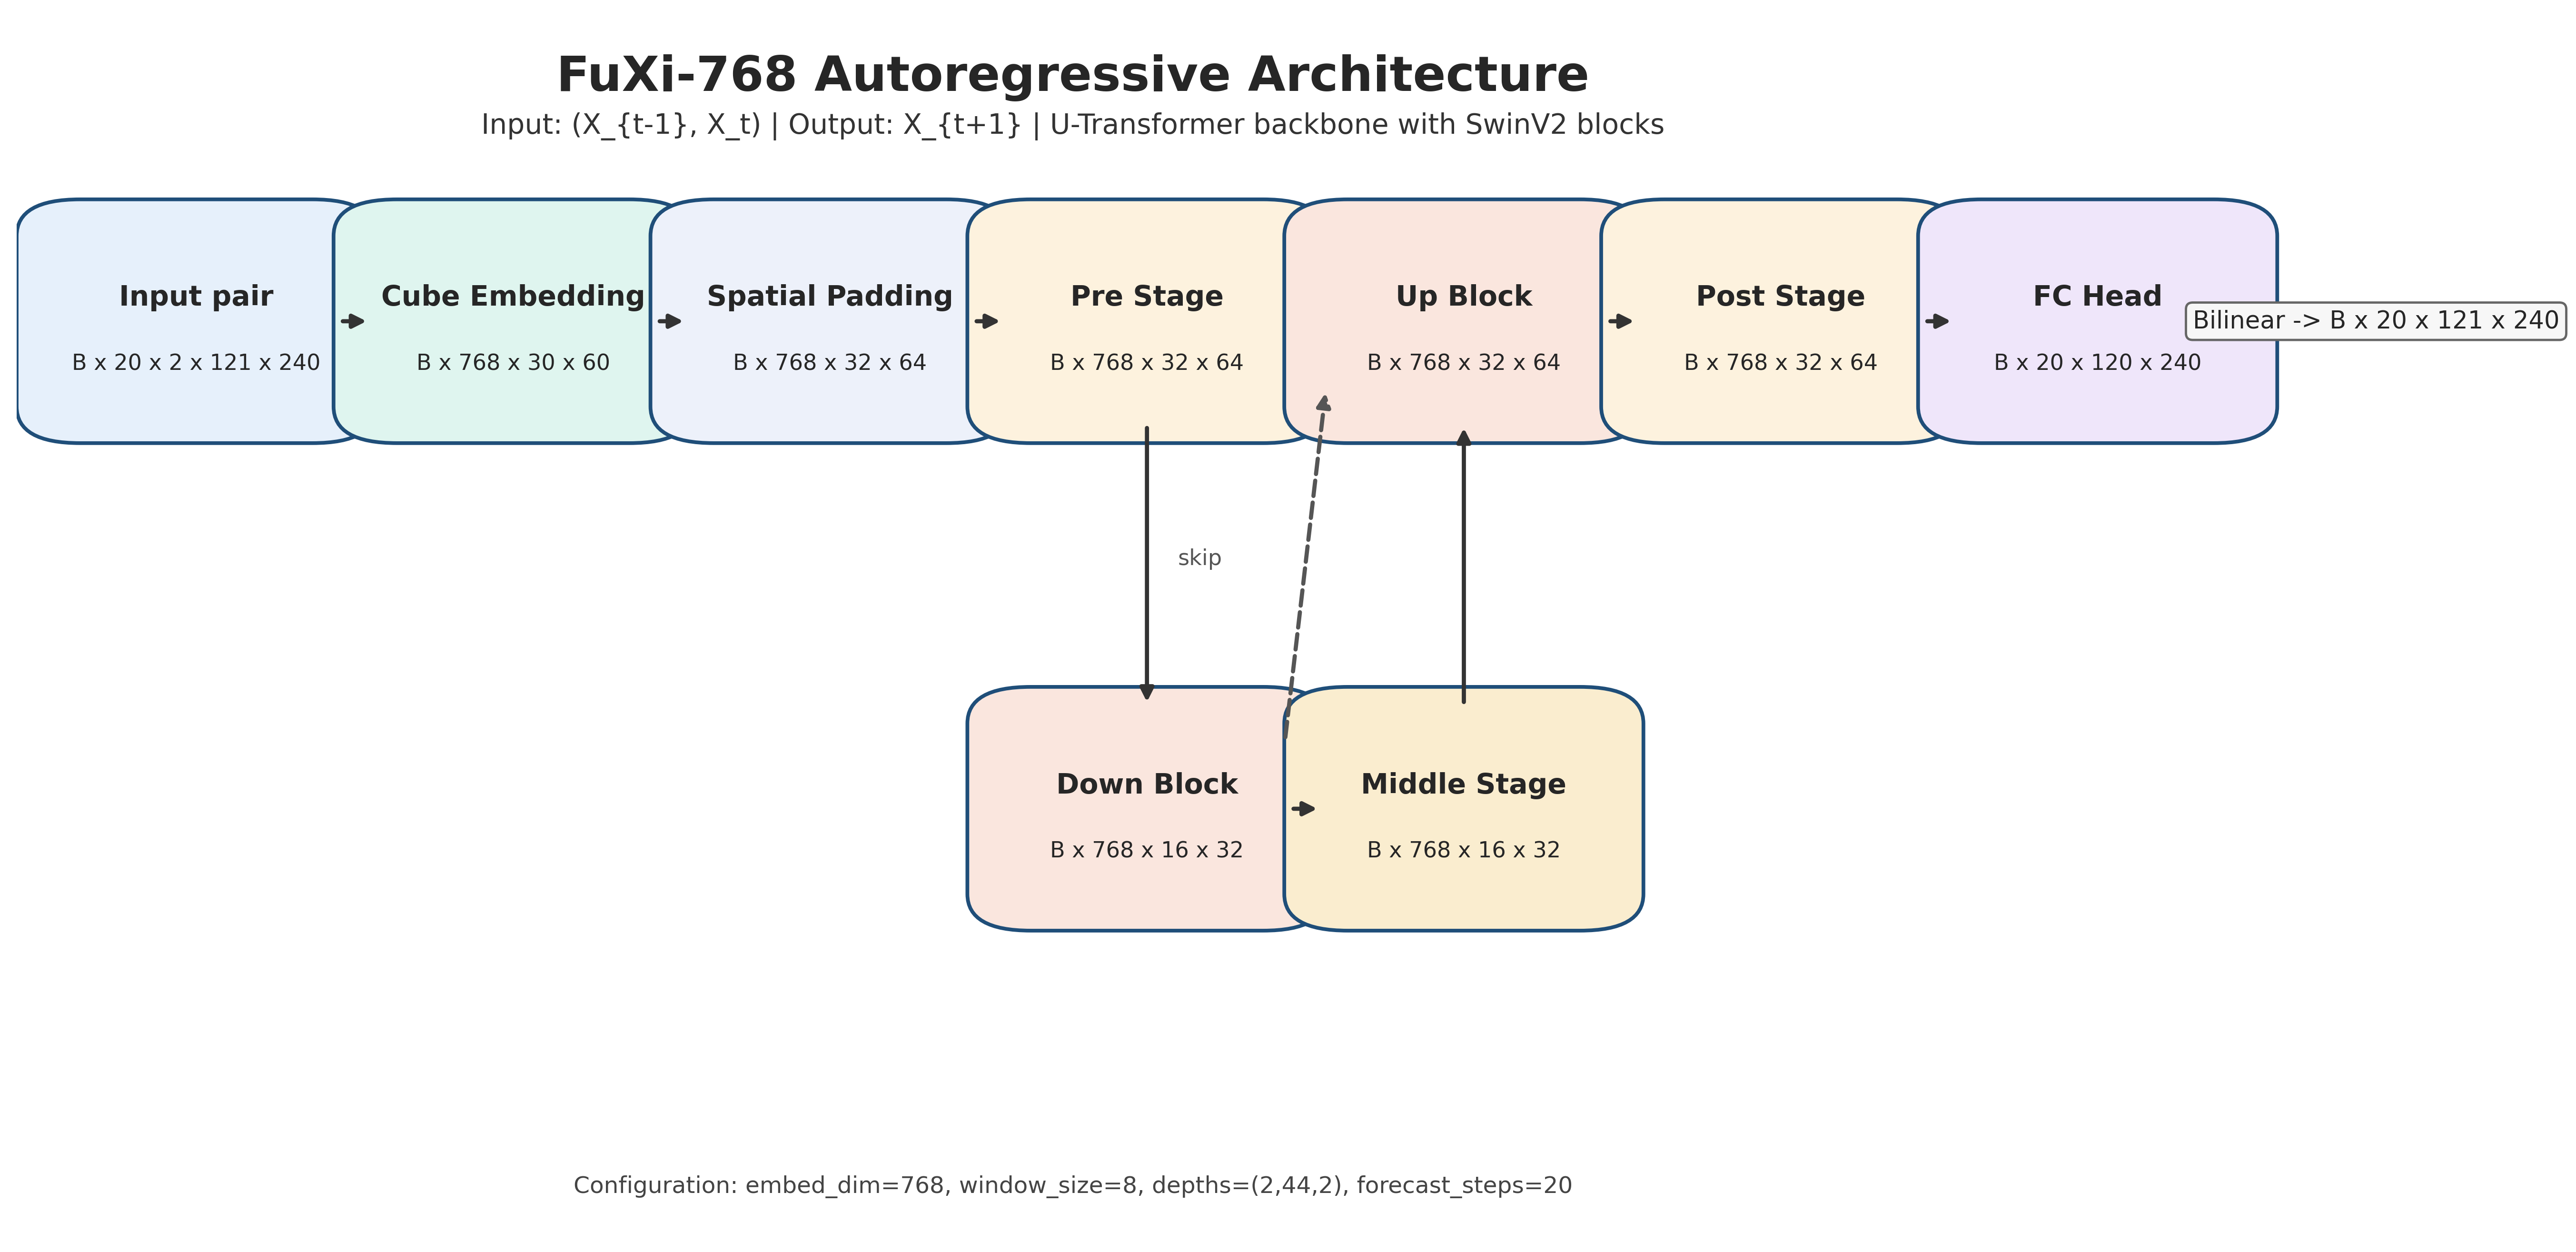
\includegraphics[width=0.92\linewidth]{arc.png}
    \caption{FuXi-inspired architecture used in this project. The model consists of cube embedding, Swin Transformer V2 encoder, U-Net-style decoder with skip connections, and final reconstruction.}
    \label{fig:fuxi_architecture}
\end{figure}

A concise description of the data flow:
\begin{enumerate}
  \item \textbf{Input:} Two consecutive timesteps → tensor of shape $(B, C=20, T=2, H=32, W=64)$.
  \item \textbf{Cube Embedding:} 3D convolutional blocks map local spatiotemporal cubes to latent tokens.
  \item \textbf{Swin Transformer V2 Encoder:} Multi-level, shifted-window self-attention extracts global context.
  \item \textbf{U-Net Decoder:} Hierarchical upsampling recovers spatial detail with skip connections.
  \item \textbf{Projection \& Interpolation:} $1\times1$ convolution + bilinear interpolation outputs 20-channel forecasts.
\end{enumerate}

\section{Why Swin + U-Net}

\begin{figure}[!htbp]
  \centering
  \begin{subfigure}[b]{0.45\textwidth}
    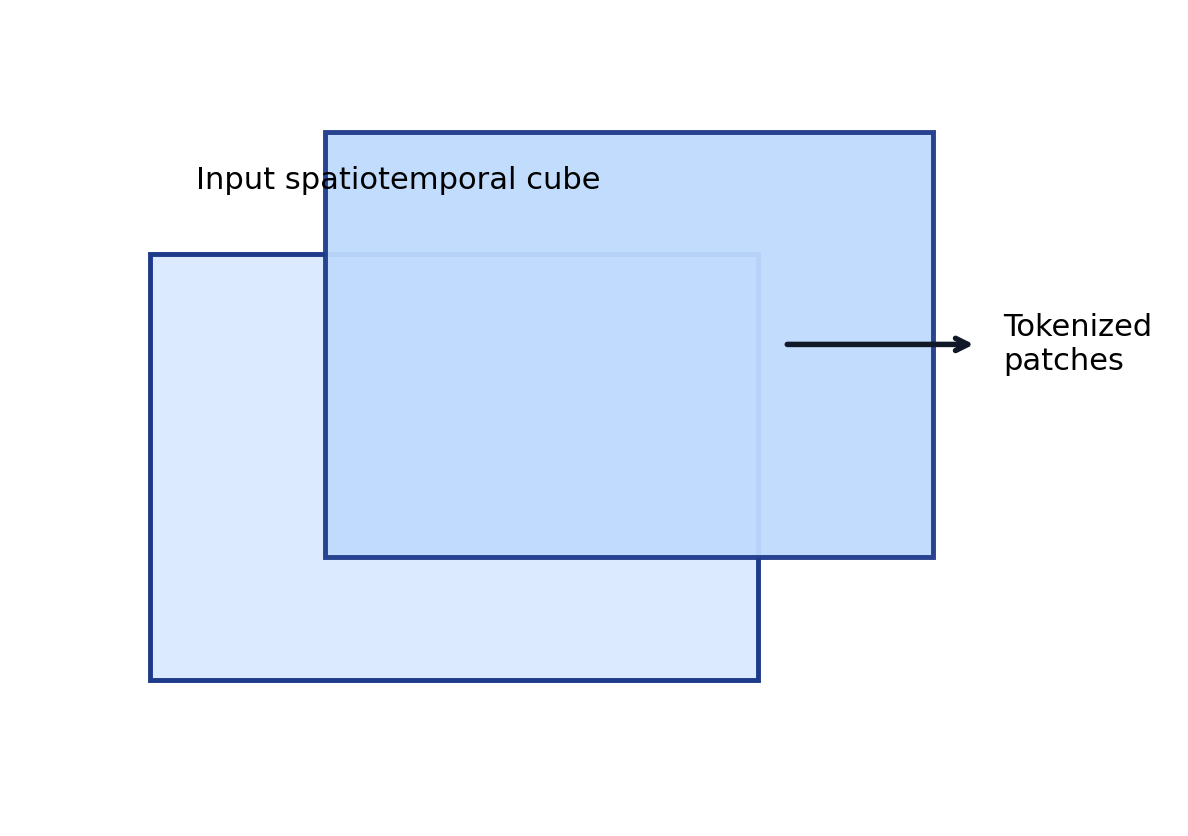
\includegraphics[width=\linewidth]{cube.png}
    \caption{Cube Embedding (3D conv)}
  \end{subfigure}
  \hfill
  \begin{subfigure}[b]{0.45\textwidth}
    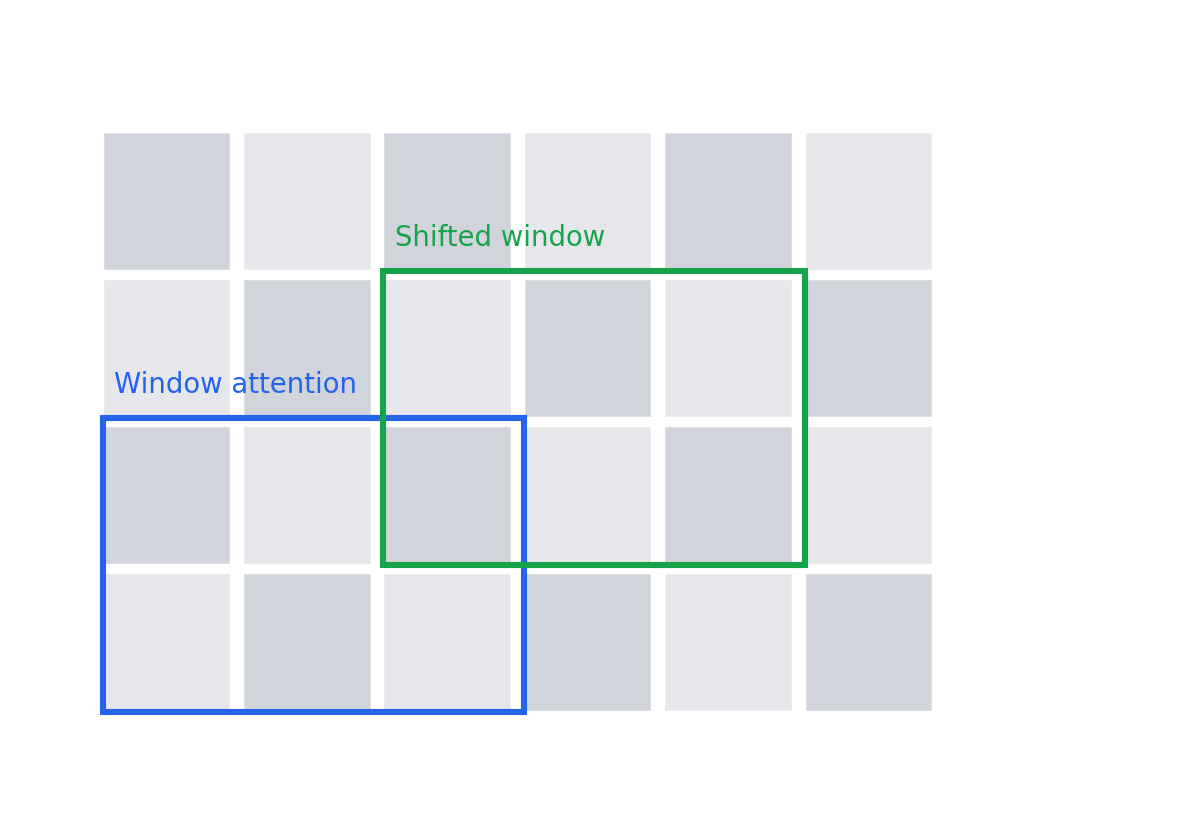
\includegraphics[width=\linewidth]{swin.png}
    \caption{Swin Transformer Block}
  \end{subfigure}

  \vspace{6pt}
  \begin{subfigure}[b]{0.7\textwidth}
    \centering
    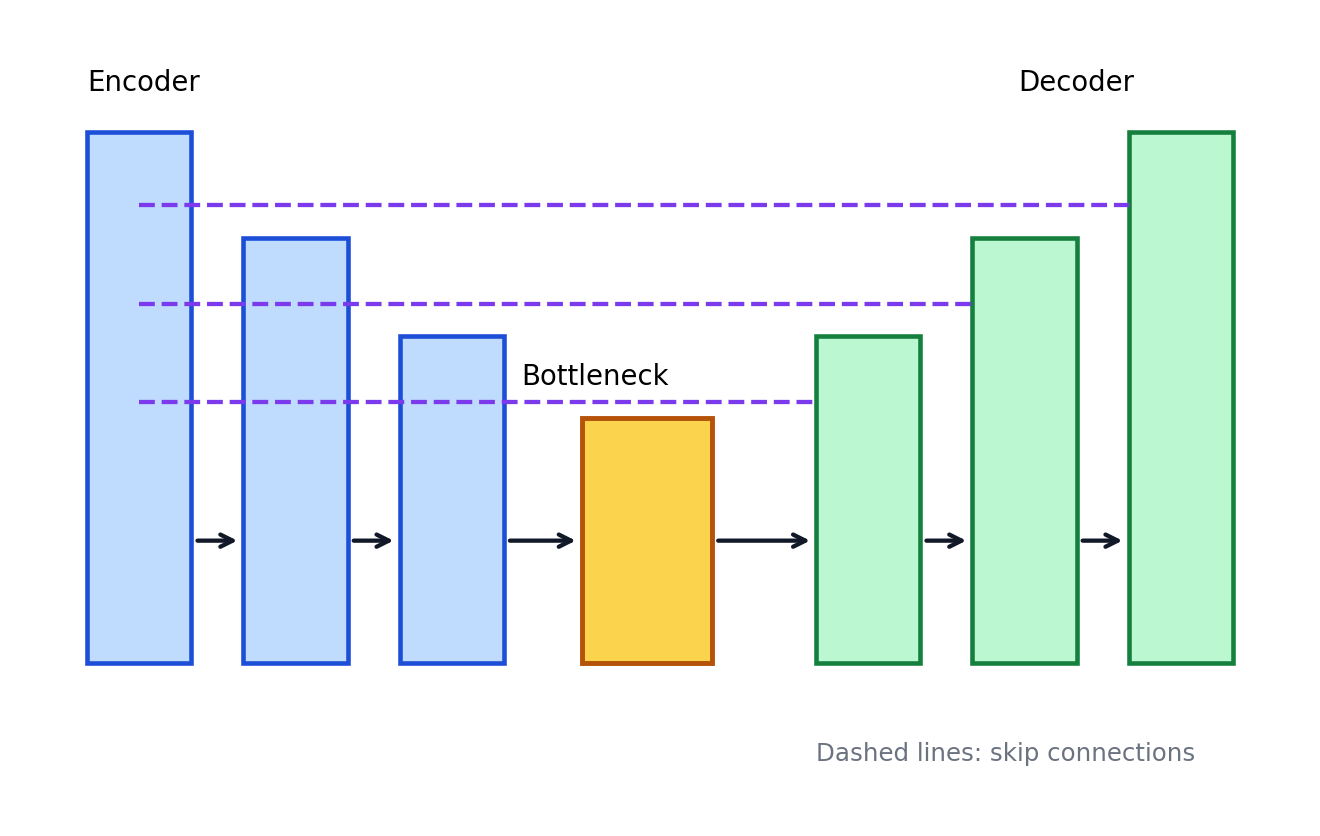
\includegraphics[width=0.55\linewidth]{unet.png}
    \caption{U-Net Decoder}
  \end{subfigure}
  \caption{Architectural building blocks.}
  \label{fig:arch_blocks}
\end{figure}

\FloatBarrier

% ---------------------------------------------------------
\chapter{Training Setup and Foundation Model Details}

We trained a foundation FuXi-like model as the starting point for this project. Key experimental settings (used to produce the foundation checkpoints referenced in this report) are listed below.

\section{Foundation Model Hyperparameters and Environment}

The foundation model was trained on NVIDIA A100 GPUs with mixed-precision (AMP). 
A small batch size was required because of the high parameter count of the Swin Transformer stacks, which quickly led to out-of-memory (OOM) conditions at the $64\times32$ resolution. 
The table below summarizes the key hyperparameters used in the first-stage FuXi-like foundation model.

\begin{table}[H]
\centering
\caption{Summary of foundation model training configuration.}
\begin{tabular}{ll}
\hline
\textbf{Setting} & \textbf{Value / Description} \\
\hline
Experiment name & \texttt{FuXi3Stage\_20251118\_005002} \\
Train / Val / Test files & 1959--2017, 2018--2020, 2021--2023 \\
Input channels & 20 variables (5 surface + 15 upper-air) \\
History steps & 2 (two consecutive timesteps as input) \\
Batch size & 2 (limited by A100 memory; deep Swin is expensive) \\
Val/Test batch size & 1 \\
Num workers & 55 (high I/O throughput on HPC cluster) \\
Max epochs & 100 with early stopping (patience = 5) \\
Learning rate & $1.5\times10^{-4}$ (AdamW) \\
Weight decay & 0.02 \\
Betas & $(0.9, 0.95)$ \\
Seed & 42 \\
Embed dimension & 512 \\
Encoder dims & (512, 768, 960) three-stage hierarchy \\
Swin depths & (3, 4, 6) blocks per stage \\
Swin heads & (8, 12, 15) multi-head attention sizes \\
Window size & 8 (shifted-window attention) \\
Drop path rate & 0.15 (regularization for deep transformers) \\
AMP & Enabled (to reduce memory footprint + faster training) \\
Resume checkpoint &
\texttt{fuxi\_epoch014.pt} (warm-start from previous run) \\
\hline
\end{tabular}
\end{table}

\paragraph{Why these choices?}
The model uses a relatively large embedding size (512) and deep Swin blocks, which dramatically increase memory consumption. Even on A100 GPUs, a batch size above 2 caused OOM errors. Using AMP helped reduce memory usage, while a high number of dataloader workers (55) ensured efficient data streaming from disk. Warm-starting from a previous checkpoint accelerated convergence and allowed exploration of architectural changes without restarting from scratch.

\noindent\textbf{Compute:} training runs used NVIDIA A100 GPUs (mixed precision/AMP enabled) and a large dataloader worker count to keep GPUs fed. The large number of workers (e.g., 55) was required during high-throughput experiments on the cluster.

\section{Training notes and observations}
\begin{itemize}
  \item \textbf{AMP and memory}: Mixed precision significantly reduced memory footprint and accelerated training, allowing larger embeddings and batch throughput.
  \item \textbf{Checkpointing}: Training resumed from the foundation checkpoint above to continue experiments; this allowed rapid iteration on architecture and loss choices.
  \item \textbf{Batch size and gradients}: Small batch sizes (2) were used due to memory constraints at this configuration; gradient noise was mitigated by appropriate learning-rate scheduling and gradient accumulation when necessary.
\end{itemize}

% ---------------------------------------------------------
\chapter{Losses and Metrics}

We used standard metrics and latitude weighting as described below.

\[
\mathcal{L}_{\text{lat-L1}}=\frac{\sum_i \cos\phi_i\,|y_i-\hat{y}_i|}{\sum_i \cos\phi_i}
\]

\[
\mathrm{RMSE}=\sqrt{\frac{1}{N}\sum_i (y_i-\hat{y}_i)^2}
\]

\[
\mathrm{ACC}=\frac{\sum_i (y_i-\bar y)(\hat{y}_i-\overline{\hat{y}})}
{\sqrt{\sum_i (y_i-\bar y)^2}\sqrt{\sum_i (\hat{y}_i-\overline{\hat{y}})^2}}
\]

\FloatBarrier

% ---------------------------------------------------------
\chapter{Results and Figures}

\begin{figure}[!htbp]
    \centering
    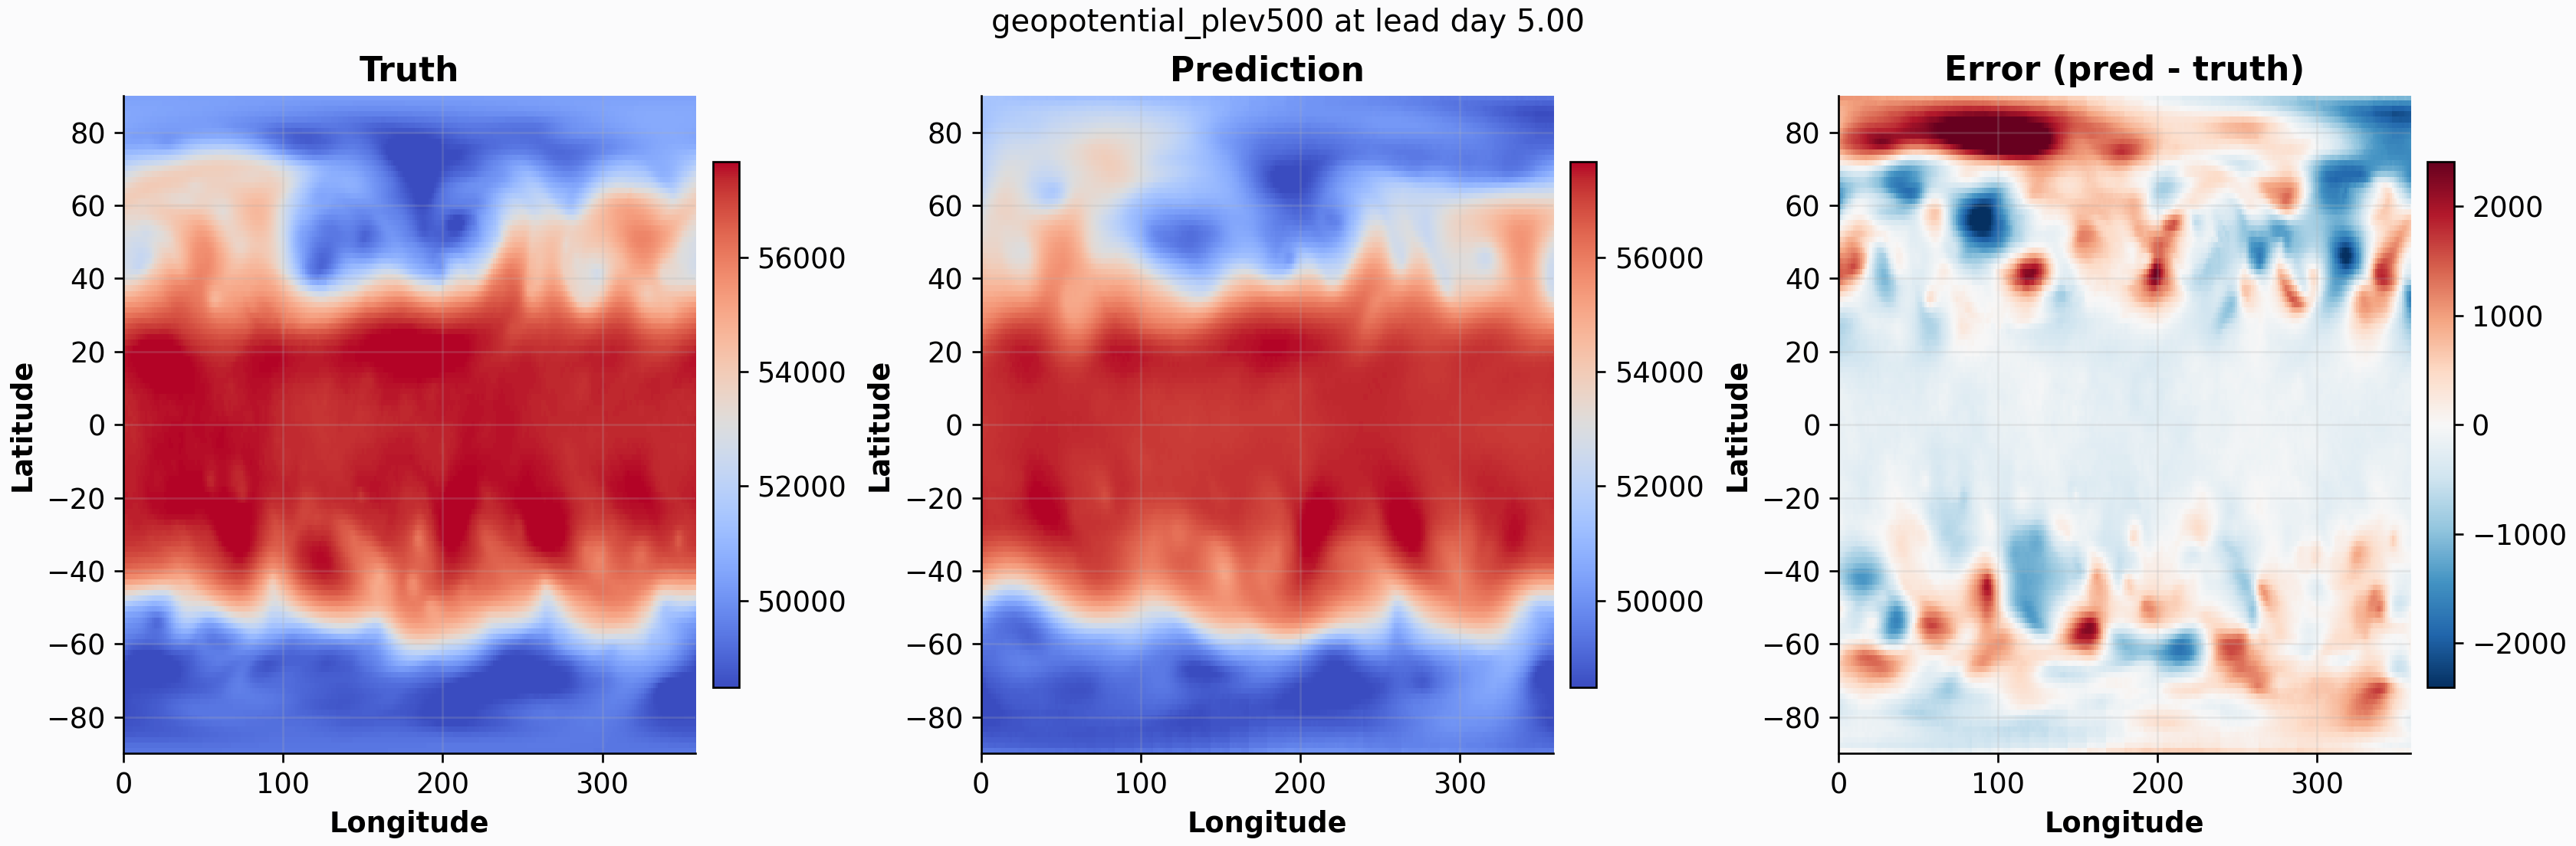
\includegraphics[width=0.65\linewidth]{target_vs_pred.png}
    \caption{Target vs Prediction--looking better then expected for me.}
    \label{fig:sixpanel}
\end{figure}

\FloatBarrier

\begin{figure}[!htbp]
  \centering
  \begin{subfigure}[b]{0.32\textwidth}
    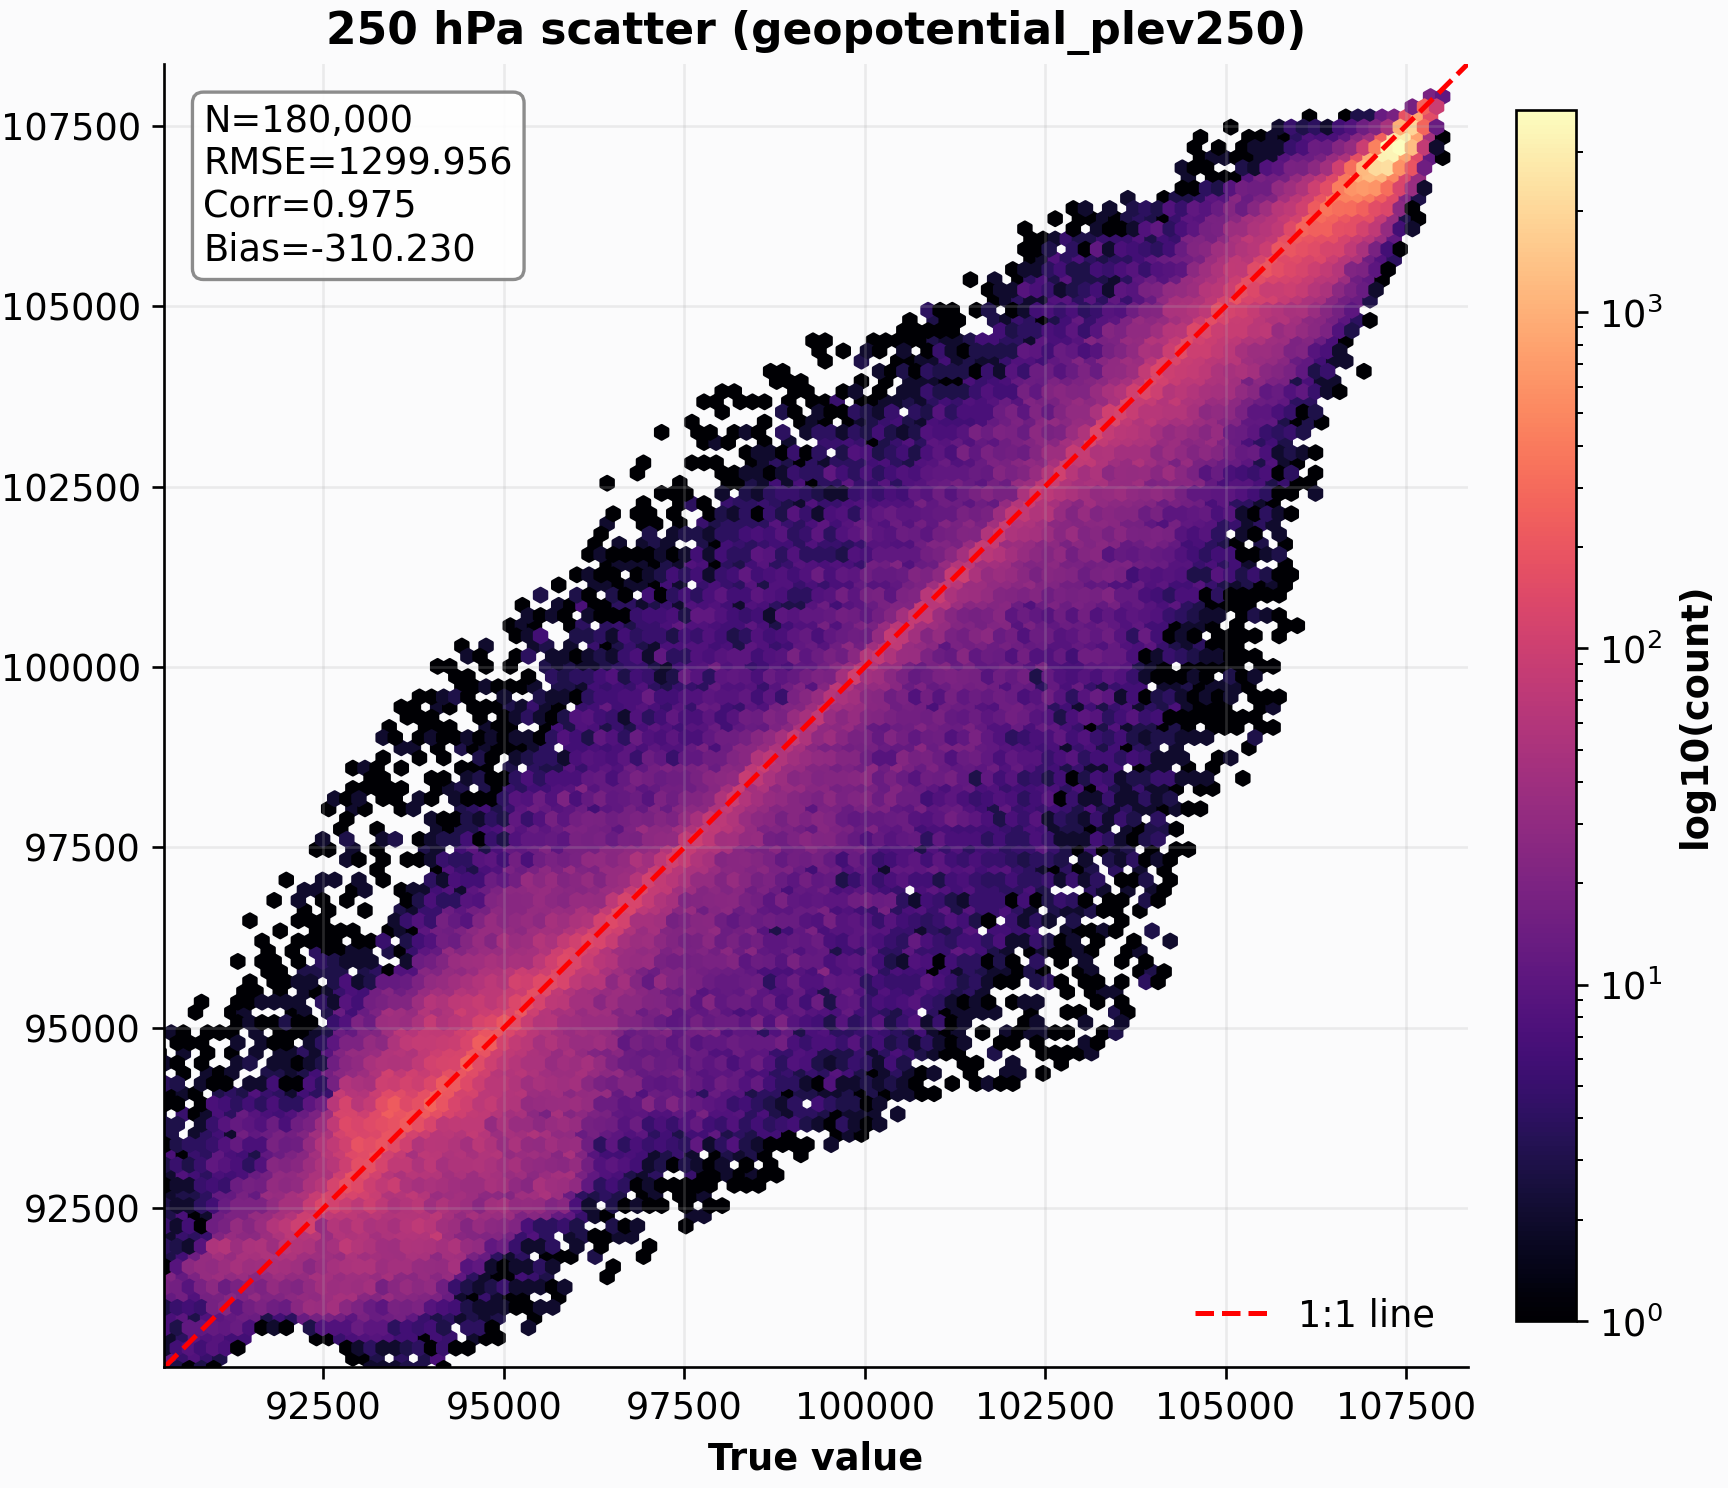
\includegraphics[width=\linewidth]{250.png}
    \caption{250 hPa}
  \end{subfigure}
  \begin{subfigure}[b]{0.32\textwidth}
    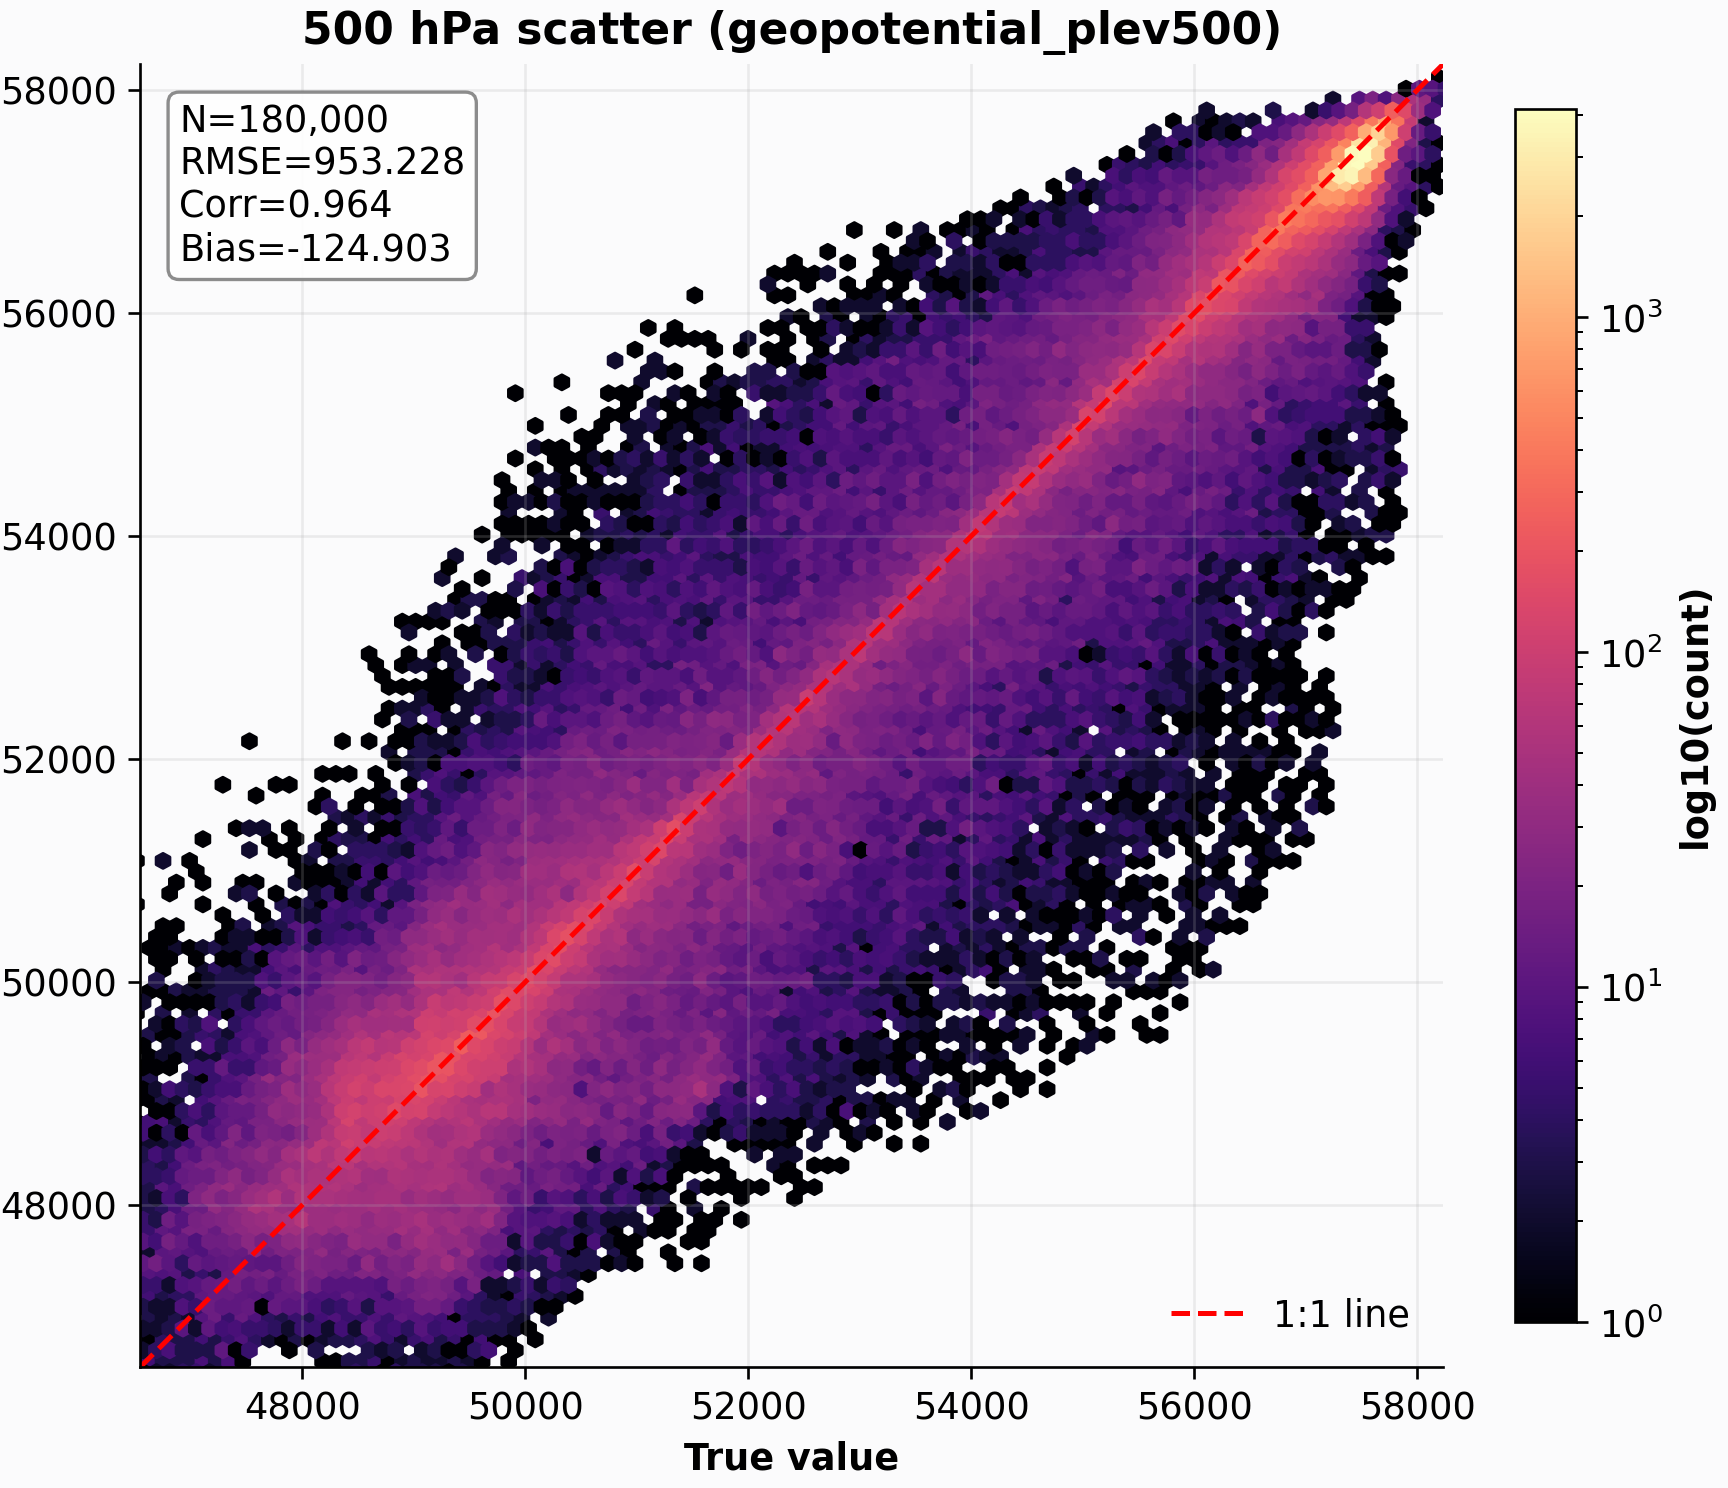
\includegraphics[width=\linewidth]{500.png}
    \caption{500 hPa}
  \end{subfigure}
  \begin{subfigure}[b]{0.32\textwidth}
    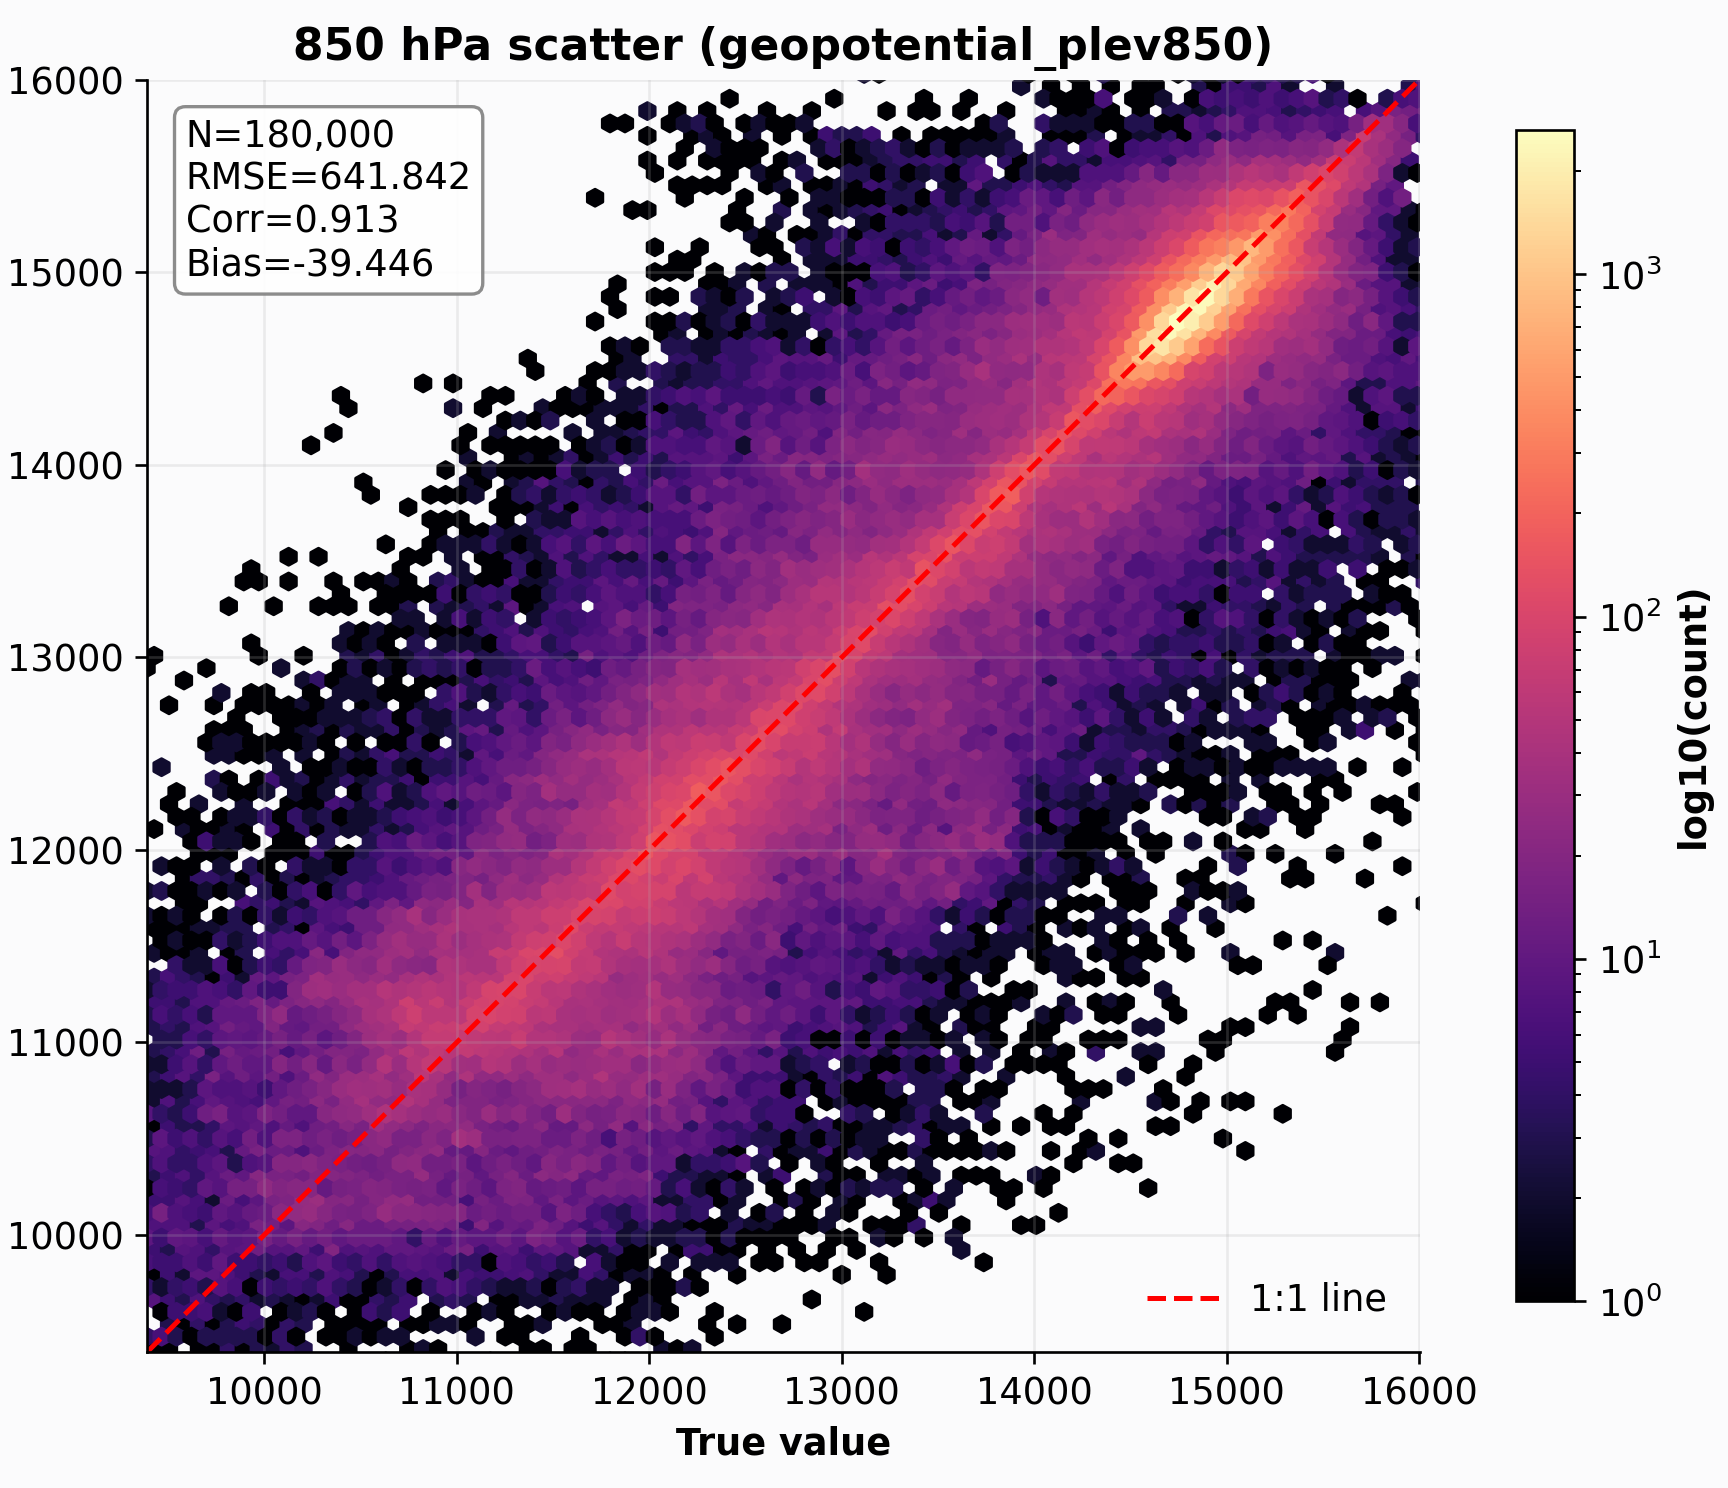
\includegraphics[width=\linewidth]{850.png}
    \caption{850 hPa}
  \end{subfigure}
  \caption{Scatter plots of predicted vs.\ true values at three pressure levels.}
  \label{fig:scatters}
\end{figure}

\FloatBarrier

\begin{figure}[!htbp]
  \centering
  \begin{subfigure}[b]{0.48\textwidth}
    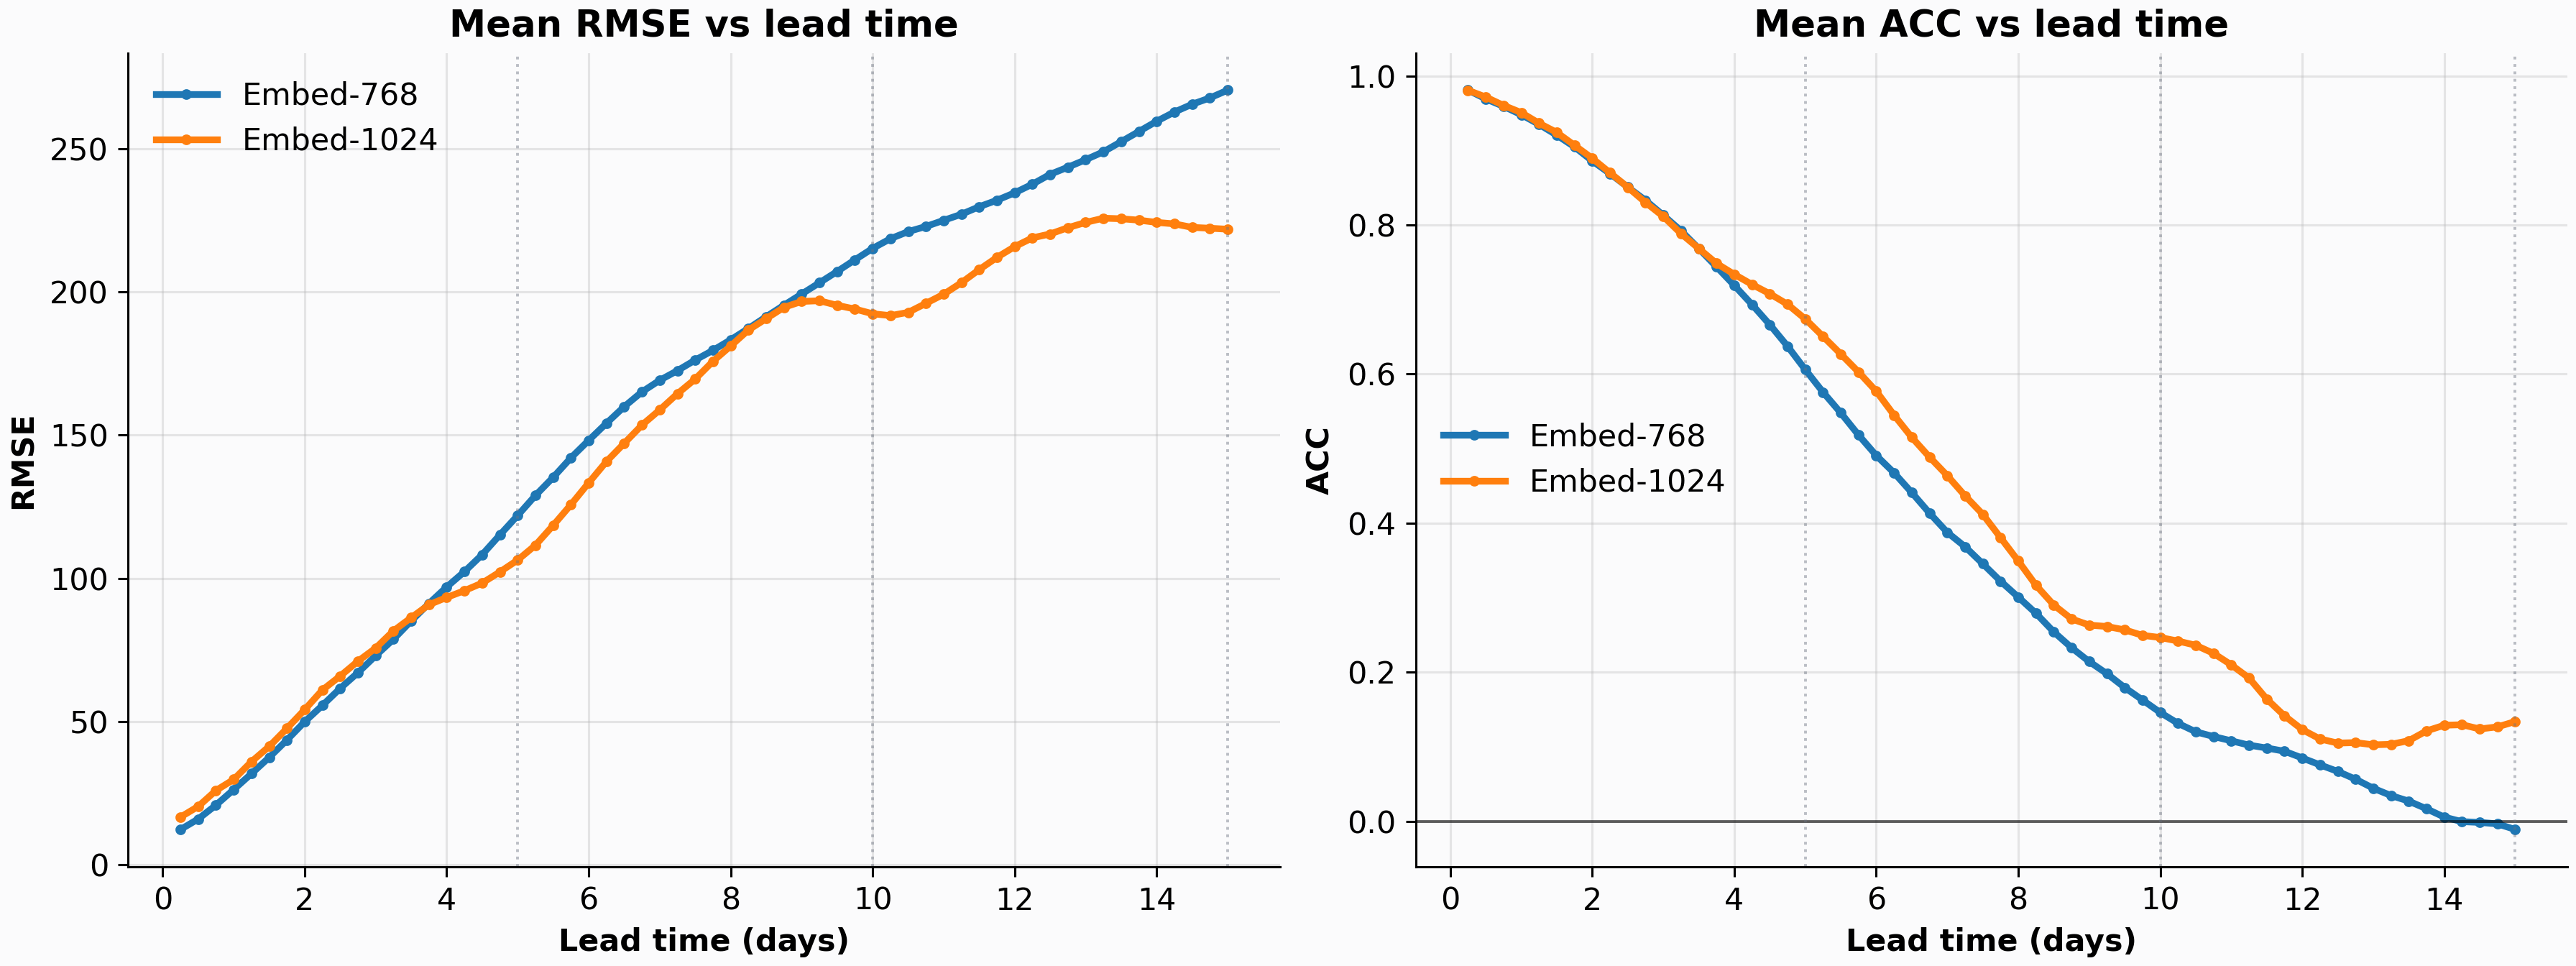
\includegraphics[width=\linewidth]{temporal_rmse.png}
    \caption{Temporal RMSE}
  \end{subfigure}
  \begin{subfigure}[b]{0.48\textwidth}
    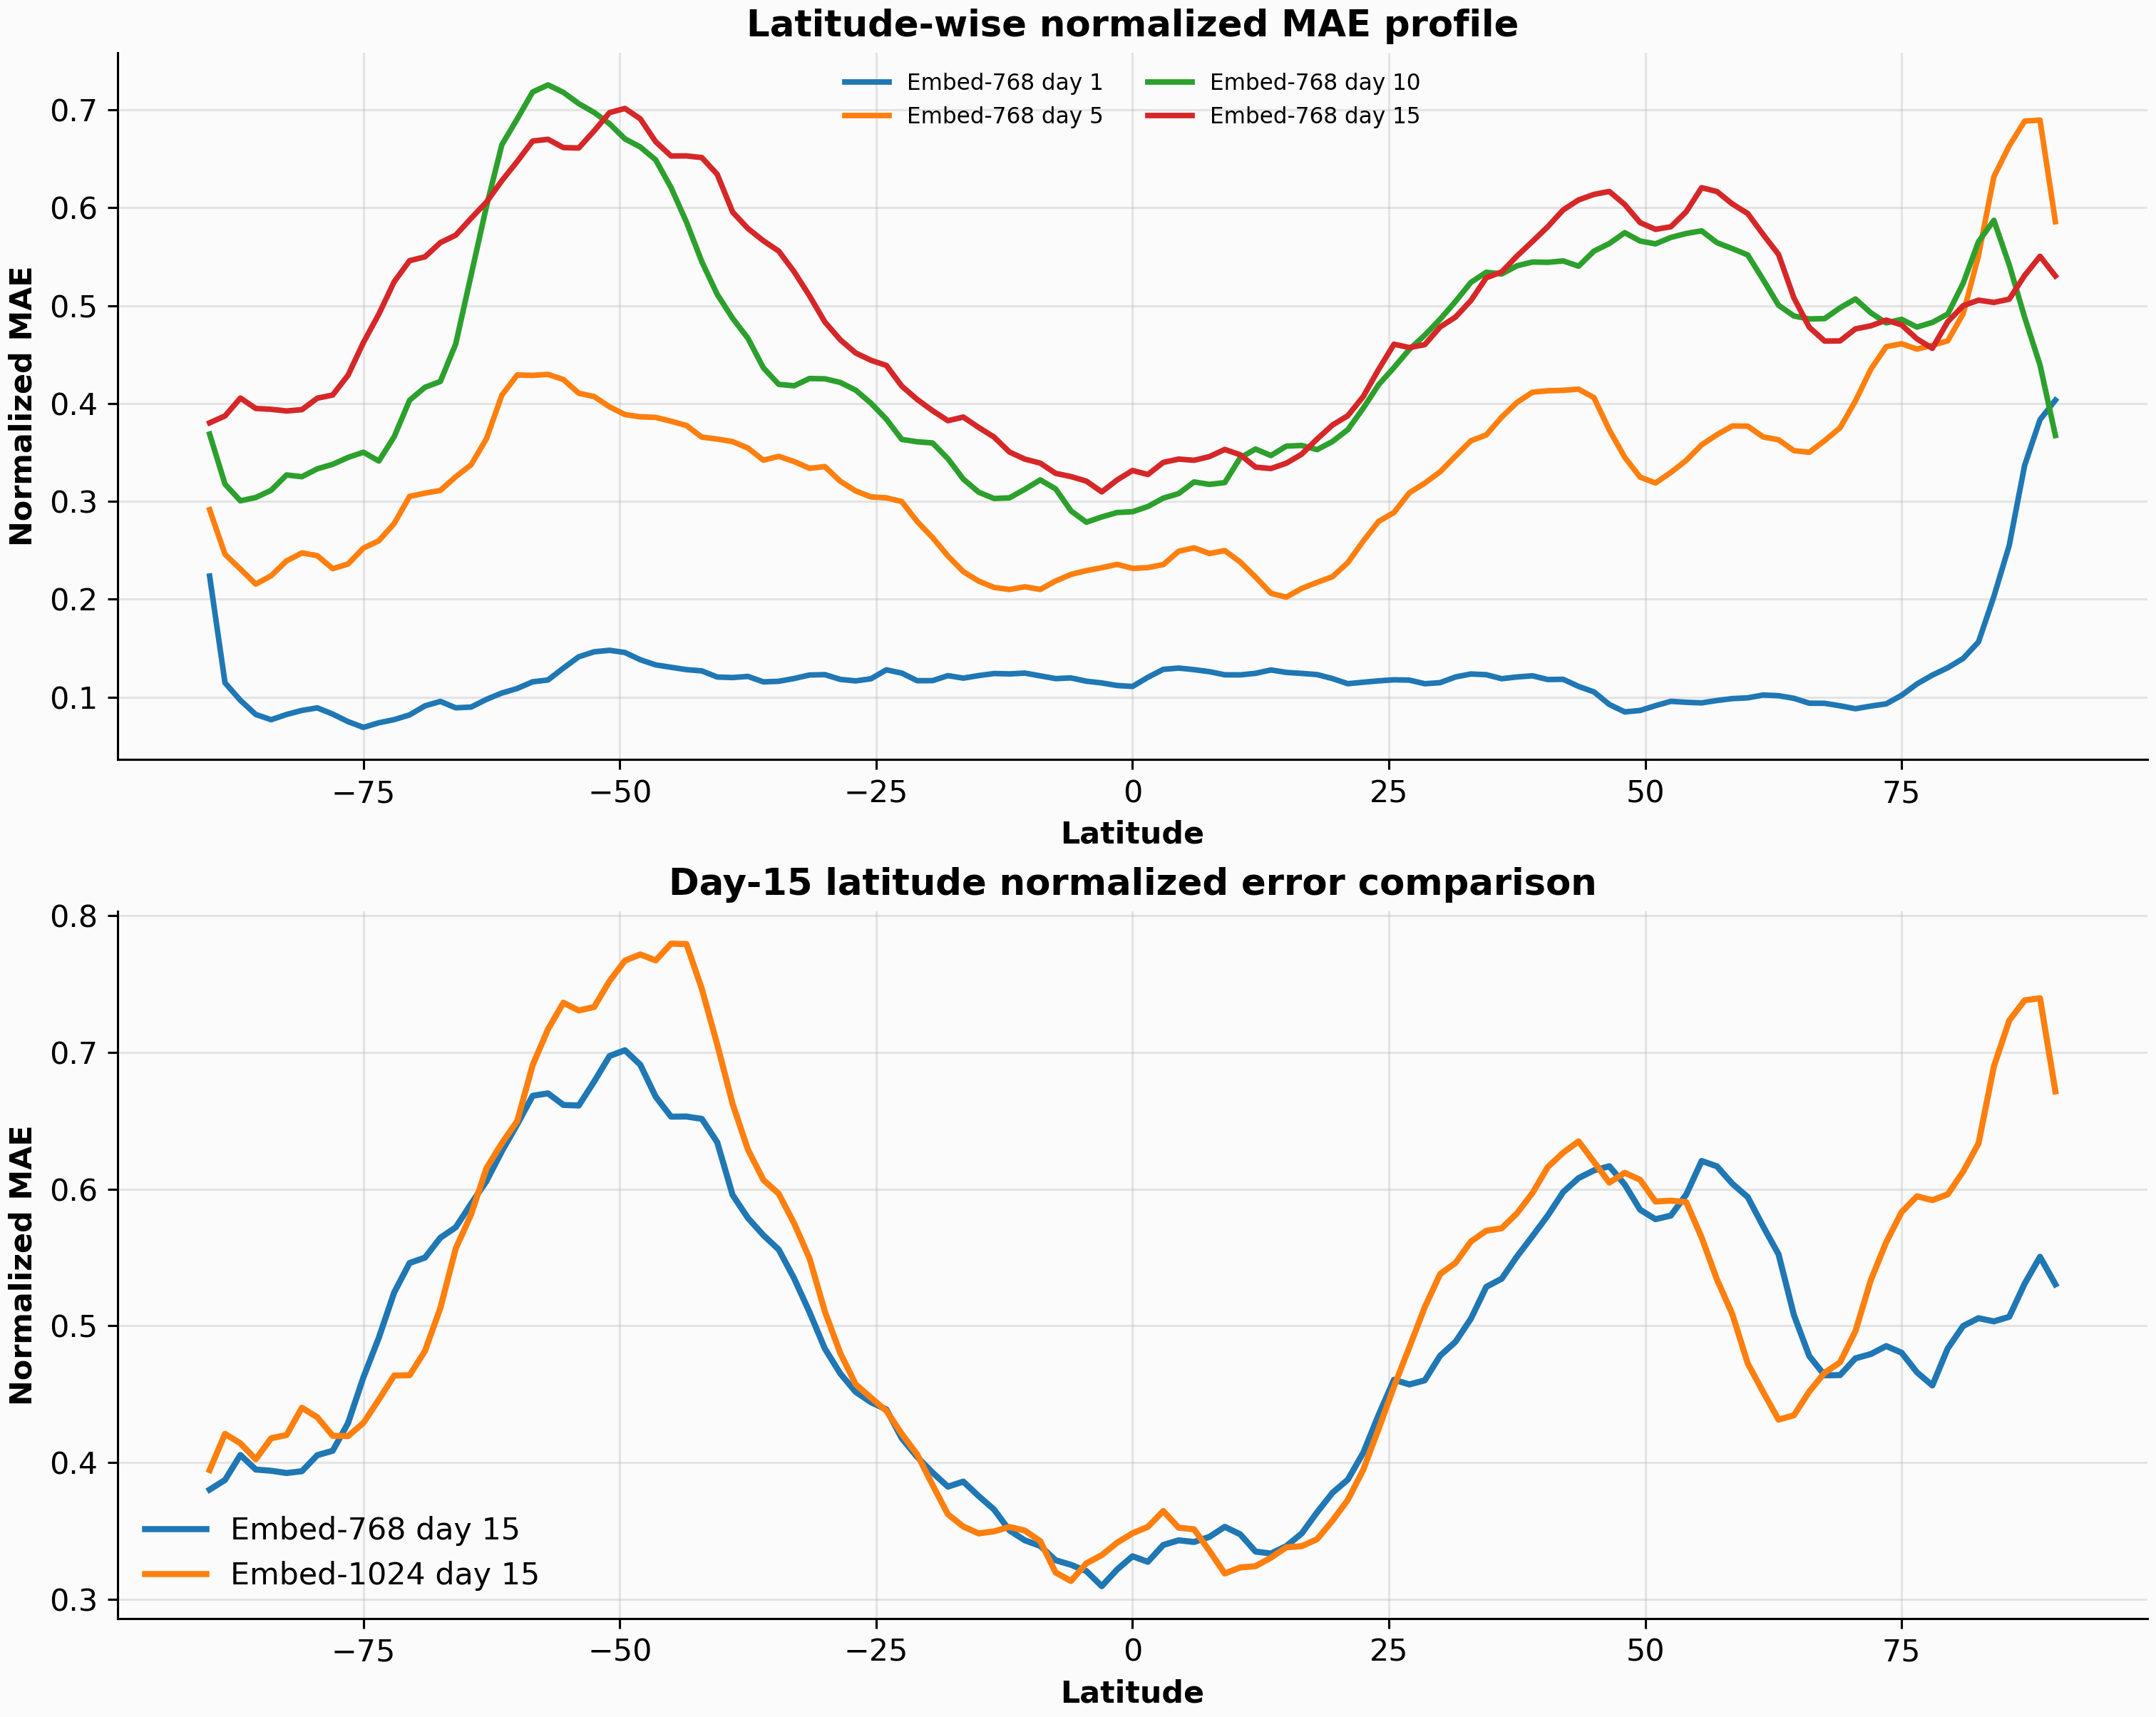
\includegraphics[width=\linewidth]{lat_err.png}
    \caption{Latitude Error Envlop}
  \end{subfigure}
  \caption{Temporal and latitudinal diagnostics.}
\end{figure}

\FloatBarrier

\begin{figure}[!htbp]
  \centering
  \begin{subfigure}[b]{0.48\textwidth}
    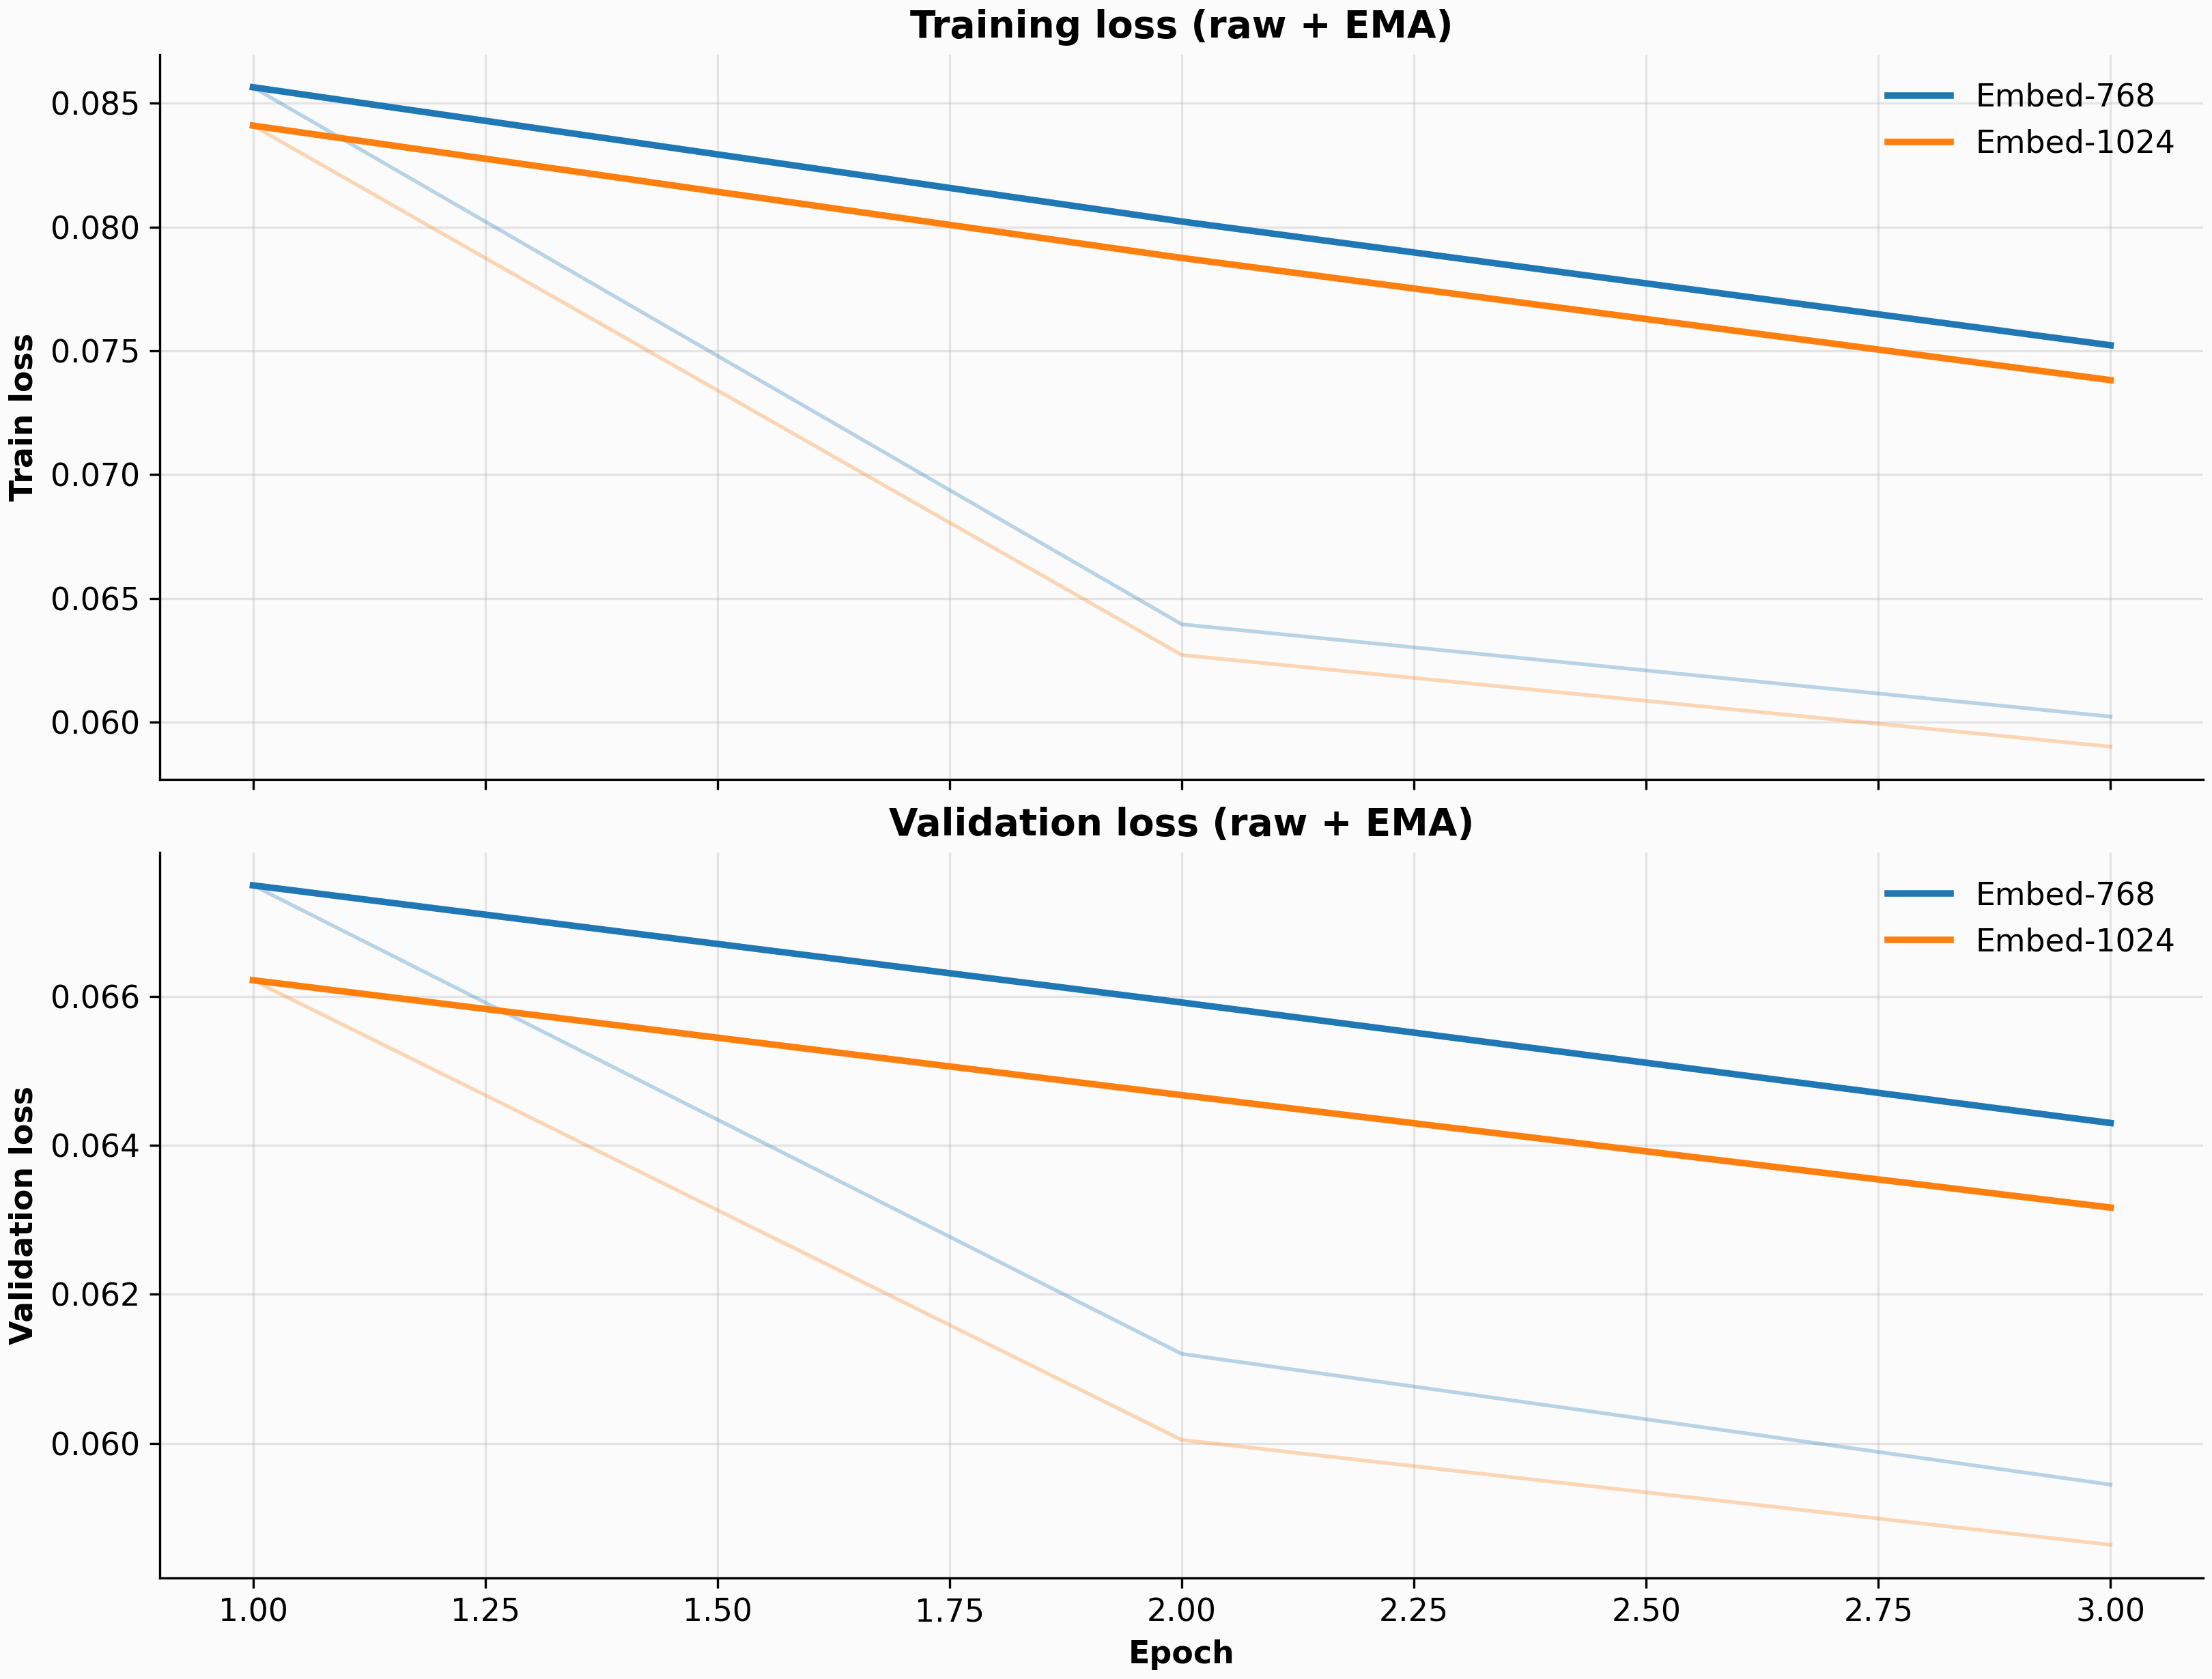
\includegraphics[width=\linewidth]{train_val.png}
    \caption{Training/Validation Loss}
  \end{subfigure}
  \begin{subfigure}[b]{0.48\textwidth}
    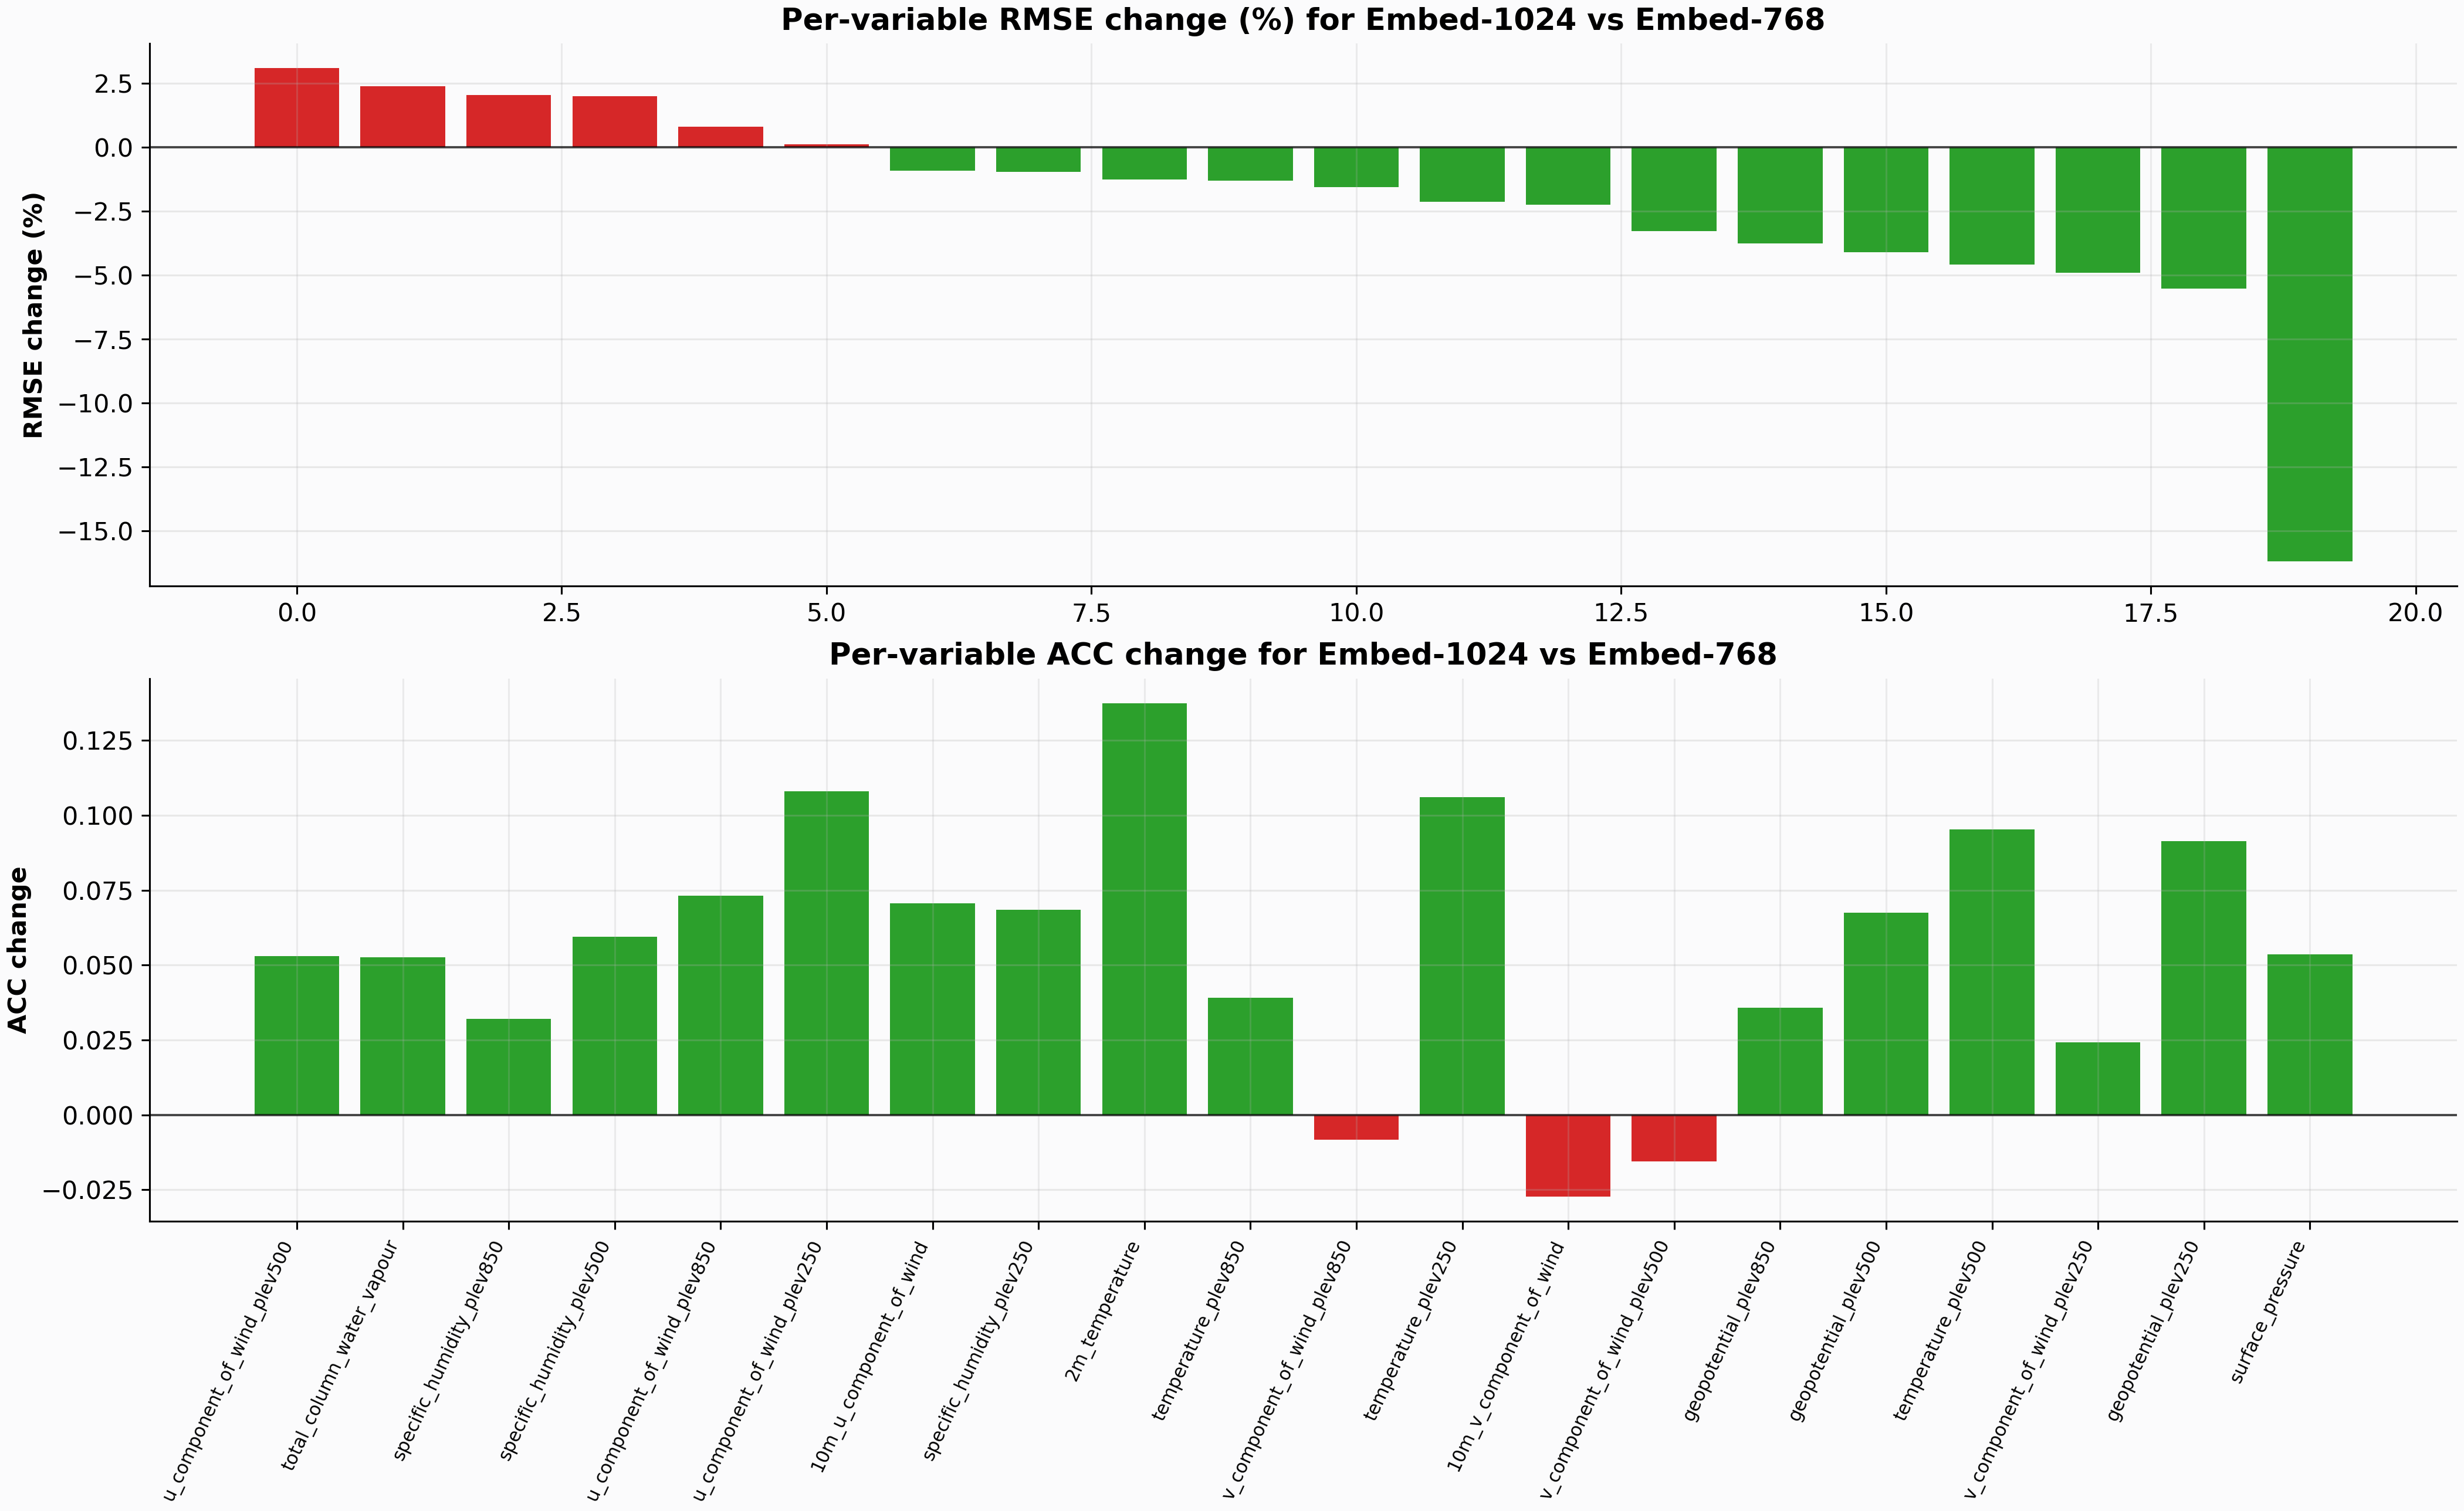
\includegraphics[width=\linewidth]{per_var_err.png}
    \caption{Per-variable Error}
  \end{subfigure}
  \caption{Training diagnostics and variable-wise performance.}
\end{figure}

\FloatBarrier

% ---------------------------------------------------------
\chapter{Challenges: Depth vs. Resolution Tradeoff}


\textbf{CODE:}\\
\url{https://github.com/Artamta/Fuxi-Weather-Prediction}\\[1.6cm]

One of the central technical observations of this work is the tradeoff between architecture depth and data resolution. At low spatial resolution (e.g., $64\times32$), deep transformer stacks (many Swin layers) can fail to learn meaningful gradients and may produce near-constant outputs — a symptom sometimes referred to as \emph{field collapse}. We observed this empirically:

\begin{itemize}
  \item \textbf{Loss of local gradients:} Downsampling strongly attenuates the small- and medium-scale features that provide the model with local gradients to learn. Attention layers operating on coarse tokens therefore receive weak, low-variance signals.
  \item \textbf{Difficulty for deep attention stacks:} Deeper Swin stacks increase representational capacity but also require informative gradients across layers. On low-resolution inputs, the gradients can vanish or fail to propagate structured spatial information, causing the network to converge to a trivial, low-variance solution.
  \item \textbf{Practical mitigation:} We found better behavior when (a) keeping the Swin depth modest, (b) complementing attention with convolutional residual blocks that preserve local structure, and (c) carefully tuning learning rates, batch sizes, and normalization. Mixed-precision training and checkpoint warm-starts also helped stabilize deeper experiments.
\end{itemize}

This tradeoff motivates the need for higher-resolution training data (1° or 0.25°) or architectural modifications (stronger convolutional inductive biases, multi-scale positional encodings) to allow deeper transformers to be effectively trained.

% ---------------------------------------------------------
\chapter{Future Work: Cascade & Autoregressive Training}

Building on FuXi’s insight, a practical route to multi-day forecasting is an autoregressive cascade of specialized models. Each model focuses on a particular lead-time window (short, medium, long), which helps prevent a single model’s errors from compounding uncontrolled across very long horizons.

\begin{figure}[!htbp]
    \centering
    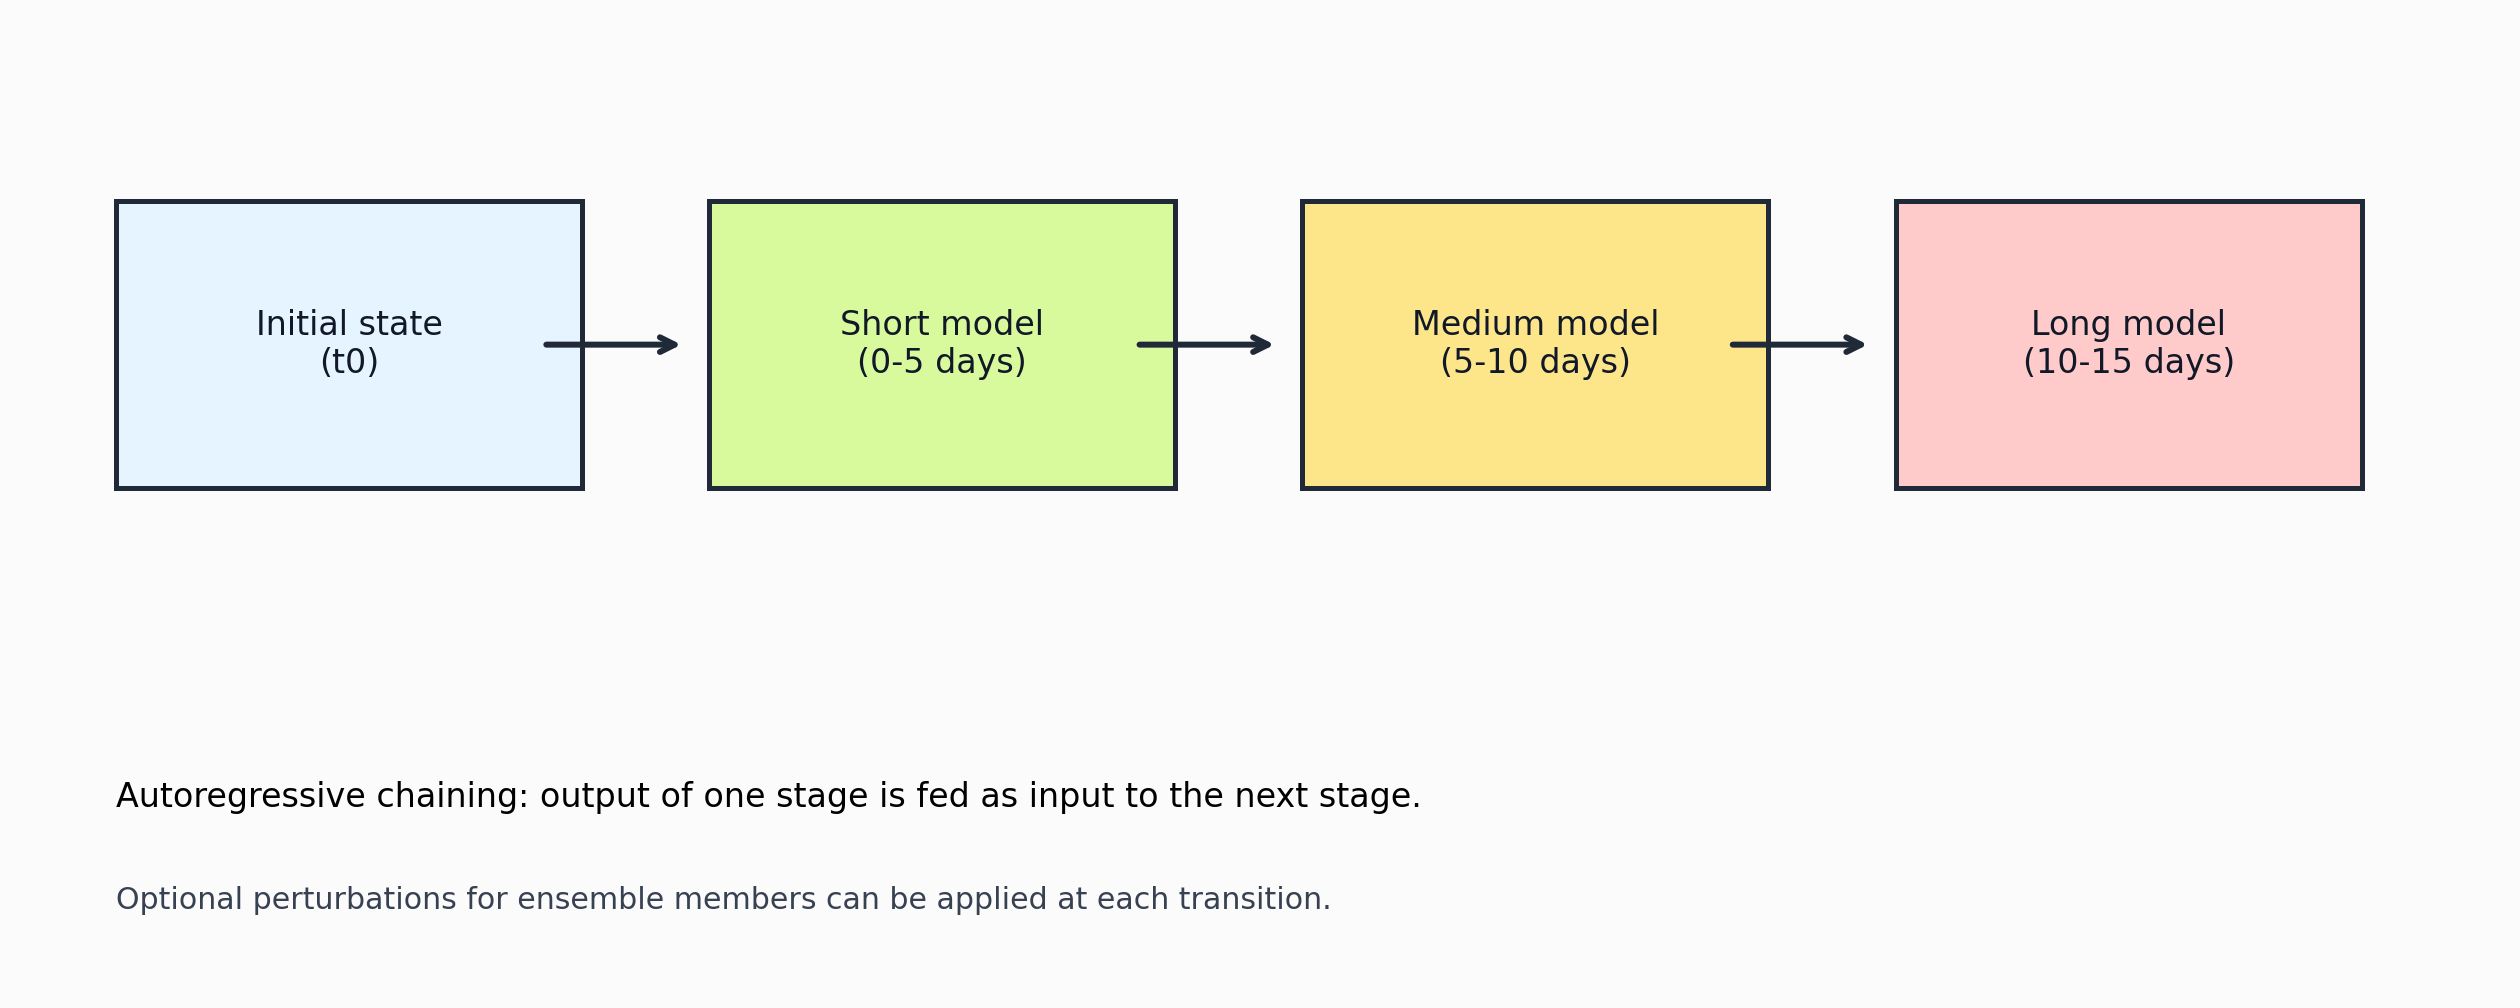
\includegraphics[width=0.85\linewidth]{cascade.png}
    \caption{FuXi-style autoregressive cascade (short/medium/long). The cascade trains specialized models for successive windows and chains them at inference time. Perlin-noise-style perturbations can be applied to generate ensemble members and stabilize training.}
    \label{fig:cascade}
\end{figure}

Planned extensions:
\begin{itemize}
  \item Train three models specialized for 0–5 d, 5–10 d, and 10–15 d; chain them autoregressively at inference time.
  \item Use small stochastic perturbations (e.g., Perlin-noise-like spatial perturbations) on initial conditions to generate ensembles and reduce sensitivity to deterministic biases.
  \item Scale training to higher resolution and deeper Swin stacks with careful warm-starting from the foundation model.
\end{itemize}

% ---------------------------------------------------------
\chapter{Practical Lessons and Final Remarks}

This project provided concrete, hands-on lessons:

\begin{itemize}
  \item \textbf{Pipeline engineering:} Building the cube embedding → Swin → U-Net pipeline reveals many practical pitfalls (shape mismatches, padding, window alignment) that are invisible in simple CV models.
  \item \textbf{Hyperparameter sensitivity:} Learning rate, batch size, and normalization choices have outsized effect on stability at low resolution.
  \item \textbf{Architecture choice:} Attention + convolution hybrids are currently the most robust design for global weather tasks, but they must be sized to match data resolution.
  \item \textbf{Compute considerations:} Training at high resolution and depth requires substantial compute (A100 or similar), careful checkpointing, and extensive tuning.
\end{itemize}

% ---------------------------------------------------------
\chapter*{Acknowledgements}

I thank Dr.~Bedartha Goswami for guidance and the IISER Pune HPC team for computational resources. I also thank the WeatherBench2 and ERA5 providers for the dataset used in this work.

% ---------------------------------------------------------
\begin{thebibliography}{9}

\bibitem{fuxi}
Chen, L. et al. (2023). \textit{FuXi: A cascade machine learning forecasting system for 15-day global weather forecast.}

\bibitem{weatherbench2}
Rasp, S. et al. (2023). \textit{WeatherBench2: A benchmark for next-generation data-driven global weather models.}

\bibitem{swin}
Liu, Z. et al. (2021). \textit{Swin Transformer: Hierarchical Vision Transformer using shifted windows.}

\bibitem{unet}
Ronneberger, O. et al. (2015). \textit{U-Net: Convolutional networks for biomedical image segmentation.}

\end{thebibliography}

\end{document}
